\documentclass[draft=false
              ,paper=a4
              ,twoside=false
              ,fontsize=11pt
              ,headsepline
              ,BCOR10mm
              ,DIV11
              ]{scrbook}
\usepackage{graphicx}
\usepackage[ngerman,english]{babel}
%% see http://www.tex.ac.uk/cgi-bin/texfaq2html?label=uselmfonts
\usepackage[T1]{fontenc}
%\usepackage[utf8]{inputenc}
\usepackage[utf8]{inputenc}
\usepackage{libertine}
\usepackage{pifont}
\usepackage{microtype}
\usepackage{textcomp}
%\usepackage[german,refpage]{nomencl}
\usepackage{setspace}
\usepackage{makeidx}
\usepackage{listings}
%\usepackage{natbib}
\usepackage[ngerman,colorlinks=true]{hyperref}
\usepackage{soul}
\usepackage{hawstyle}
\usepackage{lipsum} %% for sample text


%%%%%%%%%%%%%%%%%%%%%%%%%%%%%%%%%%%%%%%%%%%%%%%%%%%%%%%%%%%
\usepackage[backend=bibtex,bibstyle=alphabetic,citestyle=alphabetic,]{biblatex}
\addbibresource{sample.bib}
\renewcommand{\bibfootnotewrapper}[1]{%
  \bibsentence\mkbibbrackets{#1}\addperiod}
%\bibliography{sample}
\usepackage{svg}
\usepackage{amsmath}
\usepackage{xcolor}
\usepackage{fullpage}
\usepackage{tikz}
\usepackage{tikz-uml}
\usepackage[toc,acronym]{glossaries}
\usepackage[toc,page]{appendix}
\usepackage{pgfplots}
\usepackage{listings}
\def\dollar{\$}
\lstset{%
literate={my_dollar}{\$}1
%backgroundcolor=\color{gray}
}

% Appendix Name
\addto\captionsngerman{\let\appendixtocname\appendixname%
\let\appendixpagename\appendixname}

\setsvg{inkscape={"C:/Program Files/Inkscape/inkscape.exe"= -z -D}}

\tikzstyle{RectObject}=[rectangle,fill=white,draw,line width=0.5mm]
\tikzstyle{line}=[draw]
\tikzstyle{arrow}=[draw, -latex]

\newglossaryentry{repl}{
name=Read Evaluate Print Loop,
description={Pattern zum Erzeugen einer Konsole, die in einer Endlosschleife Eingaben liest, die auswertet und das Ergebnis wieder ausgibt}
}

\newglossaryentry{sla}{
name=Service Level Agreement,
description={Übereinkunft zwischen dem Anbieter und dem Nutzer eines Dienstes über dessen Qualität (z.B. Antwortzeiten, Durchsatz, Verfügbarkeit, etc.)}
}

\newacronym{tst}{TST}{Test Test Test}
%%%%%%%%%%%%%%%%%%%%%%%%%%%%%%%%%%%%%%%%%%%%%%%%%%%%%%%%%%%

%% define some colors
\colorlet{BackgroundColor}{gray!20}
\colorlet{KeywordColor}{blue}
\colorlet{CommentColor}{black!60}
%% for tables
\colorlet{HeadColor}{gray!60}
\colorlet{Color1}{blue!10}
\colorlet{Color2}{white}

%% configure colors
\HAWifprinter{
  \colorlet{BackgroundColor}{gray!20}
  \colorlet{KeywordColor}{black}
  \colorlet{CommentColor}{gray}
  % for tables
  \colorlet{HeadColor}{gray!60}
  \colorlet{Color1}{gray!40}
  \colorlet{Color2}{white}
}{}
\lstset{%
  numbers=left,
  numberstyle=\tiny,
  stepnumber=1,
  numbersep=5pt,
  basicstyle=\ttfamily\small,
  keywordstyle=\color{KeywordColor}\bfseries,
  identifierstyle=\color{black},
  commentstyle=\color{CommentColor},
  backgroundcolor=\color{BackgroundColor},
  captionpos=b,
  fontadjust=true
}
\lstset{escapeinside={(*@}{@*)}, % used to enter latex code inside listings
        morekeywords={uint32_t, int32_t}
}
\ifpdfoutput{
  \hypersetup{bookmarksopen=false,bookmarksnumbered,linktocpage}
}{}


%% more fancy C++
\DeclareRobustCommand{\cxx}{C\raisebox{0.25ex}{{\scriptsize +\kern-0.25ex +}}}

\clubpenalty=10000
\widowpenalty=10000
\displaywidowpenalty=10000

% unknown hyphenations
\hyphenation{
}

%% recalculate text area
\typearea[current]{last}

\makeindex
%\makenomenclature
\makeglossaries

\begin{document}
\selectlanguage{ngerman}

%%%%%
%% customize (see readme.pdf for supported values)
\HAWThesisProperties{Author={Daniel Kirchner}
                    ,Title={Skalierbare Datenanalyse mit Apache Spark}
										,SubTitle={Implementation einer Text-Mining-Anwendung und Betrieb auf einem Low-End-Cluster}
                    ,EnglishTitle={Scalable Data Analysis with Apache Spark}
                    ,ThesisType={Bachelorarbeit}
                    ,ExaminationType={Bachelorprüfung}
                    ,DegreeProgramme={Bachelor of Science Angewandte Informatik}
                    ,ThesisExperts={Prof. Dr. Kahlbrandt \and Prof. Dr. Zukunft}
                    ,ReleaseDate={17. Juni 2015}
                  }

%% title
\frontmatter

%% output title page
\maketitle

\onehalfspacing

%% add abstract pages
%% note: this is one command on multiple lines
\HAWAbstractPage
%% German abstract
{Apache Spark, Big Data, Architekturanalyse, Text Mining, Echtzeit-Datenanalyse, Raspberry Pi}%
{Apache Spark ist auf dem Weg sich als zentrale Komponente von Big-Data-Analyse-Systemen für eine Vielzahl von Anwendungsfällen durchzusetzen. Diese Arbeit schafft einen Überblick der zentralen Konzepte und Bestandteile von Apache Spark und untersucht das Verhalten von Spark auf einem Cluster mit minimalem Leistungsprofil. Grundlage dieser Untersuchung ist ein realitätsnaher Anwendungsfall, der Sparkmodule für Batch-Processing und Streaming kombiniert.}
%% English abstract
{keyword 1, keyword 2}%
{This document \ldots}

\newpage
\singlespacing

\tableofcontents

\newpage
%% enable if these lists should be shown on their own page
\listoffigures
\listoftables
\lstlistoflistings

%% main
\mainmatter
\onehalfspacing
%% write to the log/stdout
\typeout{===== Chapter Files}
\chapter{Einführung}

\section{Motivation}

Die Entwicklung und Verbesserung von Frameworks zur Verarbeitung großer Datenmengen ist zur Zeit hochaktuell und zunehmend im Fokus von Medien und Unternehmen. Verschiedene Programme und Paradigmen konkurrieren um die schnellste, bequemste und stabilste Art großen Datenmengen einen geschäftsfördernden Nutzen abzuringen \cite{Sin14}.\\

Mit dem Begriff "`große Datenmengen"' oder "`Big Data"' werden in dieser Arbeit solche Datenmengen zusammengefasst, die die Kriterien Volume, Velocity, Variety \footcite{Lan01} erfüllen oder "`Datenmengen, die nicht mehr unter Auflage bestimmter \gls{sla}s auf einzelnen Maschinen verarbeitet werden können"' (Vgl. \cite{Sam14}).\\

Als Unternehmen, das früh mit zeitkritischen Aufgaben (u.a.  Indizierung von Webseiten und PageRank \footcite{page2001method}) auf solchen Datenmengen konfrontiert war implementierte Google das Map-Reduce Paradigma \footcite{Dean04} als Framework zur Ausnutzung vieler kostengünstiger Rechner für verschiedene Aufgaben. \\

In Folge der Veröffentlichung dieser Idee im Jahr 2004 wurde Map-Reduce in Form der OpenSource Implementation Hadoop (gemeinsam mit einer Implementation des Google File Systems GFS, u.a.) \footcite{Ghema03} zum de-facto Standard für Big-Data-Analyseaufgaben.\\

Reines Map-Reduce (nach Art von Hadoop) als Programmierparadigma zur Verarbeitung großer Datenmengen zeigt jedoch in vielen Anwendungsfällen Schwächen:
\begin{itemize}
	\item Daten, die in hoher Frequenz entstehen und schnell verarbeitet werden sollen erfordern häufiges Neustarten von Map-Reduce-Jobs. Die Folge ist kostspieliger Overhead durch Verwaltung/Scheduling der Jobs und gegebenenfalls wiederholtem Einlesen von Daten.
	\item Algorithmen die während ihrer Ausführung iterativ Zwischenergebnisse erzeugen und auf vorherige angewiesen sind (häufig bei Maschinenlernalgorithmen) können nur durch persistentes Speichern der Daten und wiederholtes Einlesen zwischen allen Iterationsschritten implementiert werden.
	\item Anfragen an ein solches Map-Reduce-System erfolgen imperativ in Form von kleinen Programmen. Dieses Verfahren ist offensichtlich nicht so intuitiv und leicht erlernbar wie deklarative Abfragesprachen klassischer Datenbanken (z.B. SQL).
\end{itemize}

In der Folge dieser Probleme entstanden viele Ansätze dieses Paradigma zu ersetzen, zu ergänzen oder durch übergeordnete Ebenen und High-Level-APIs zu vereinfachen \footcite{Sin14}.\\

Eine der Alternativen zu der klassischen Map-Reduce-Komponente in Hadoop ist die "`general engine for large-scale data processing"' Apache Spark.\\

Ein Indiz für das steigende Interesse an diesem Produkt liefert unter anderem ein Vergleich des Interesses an Hadoop und Spark auf Google:\\

\begin{figure}[h]
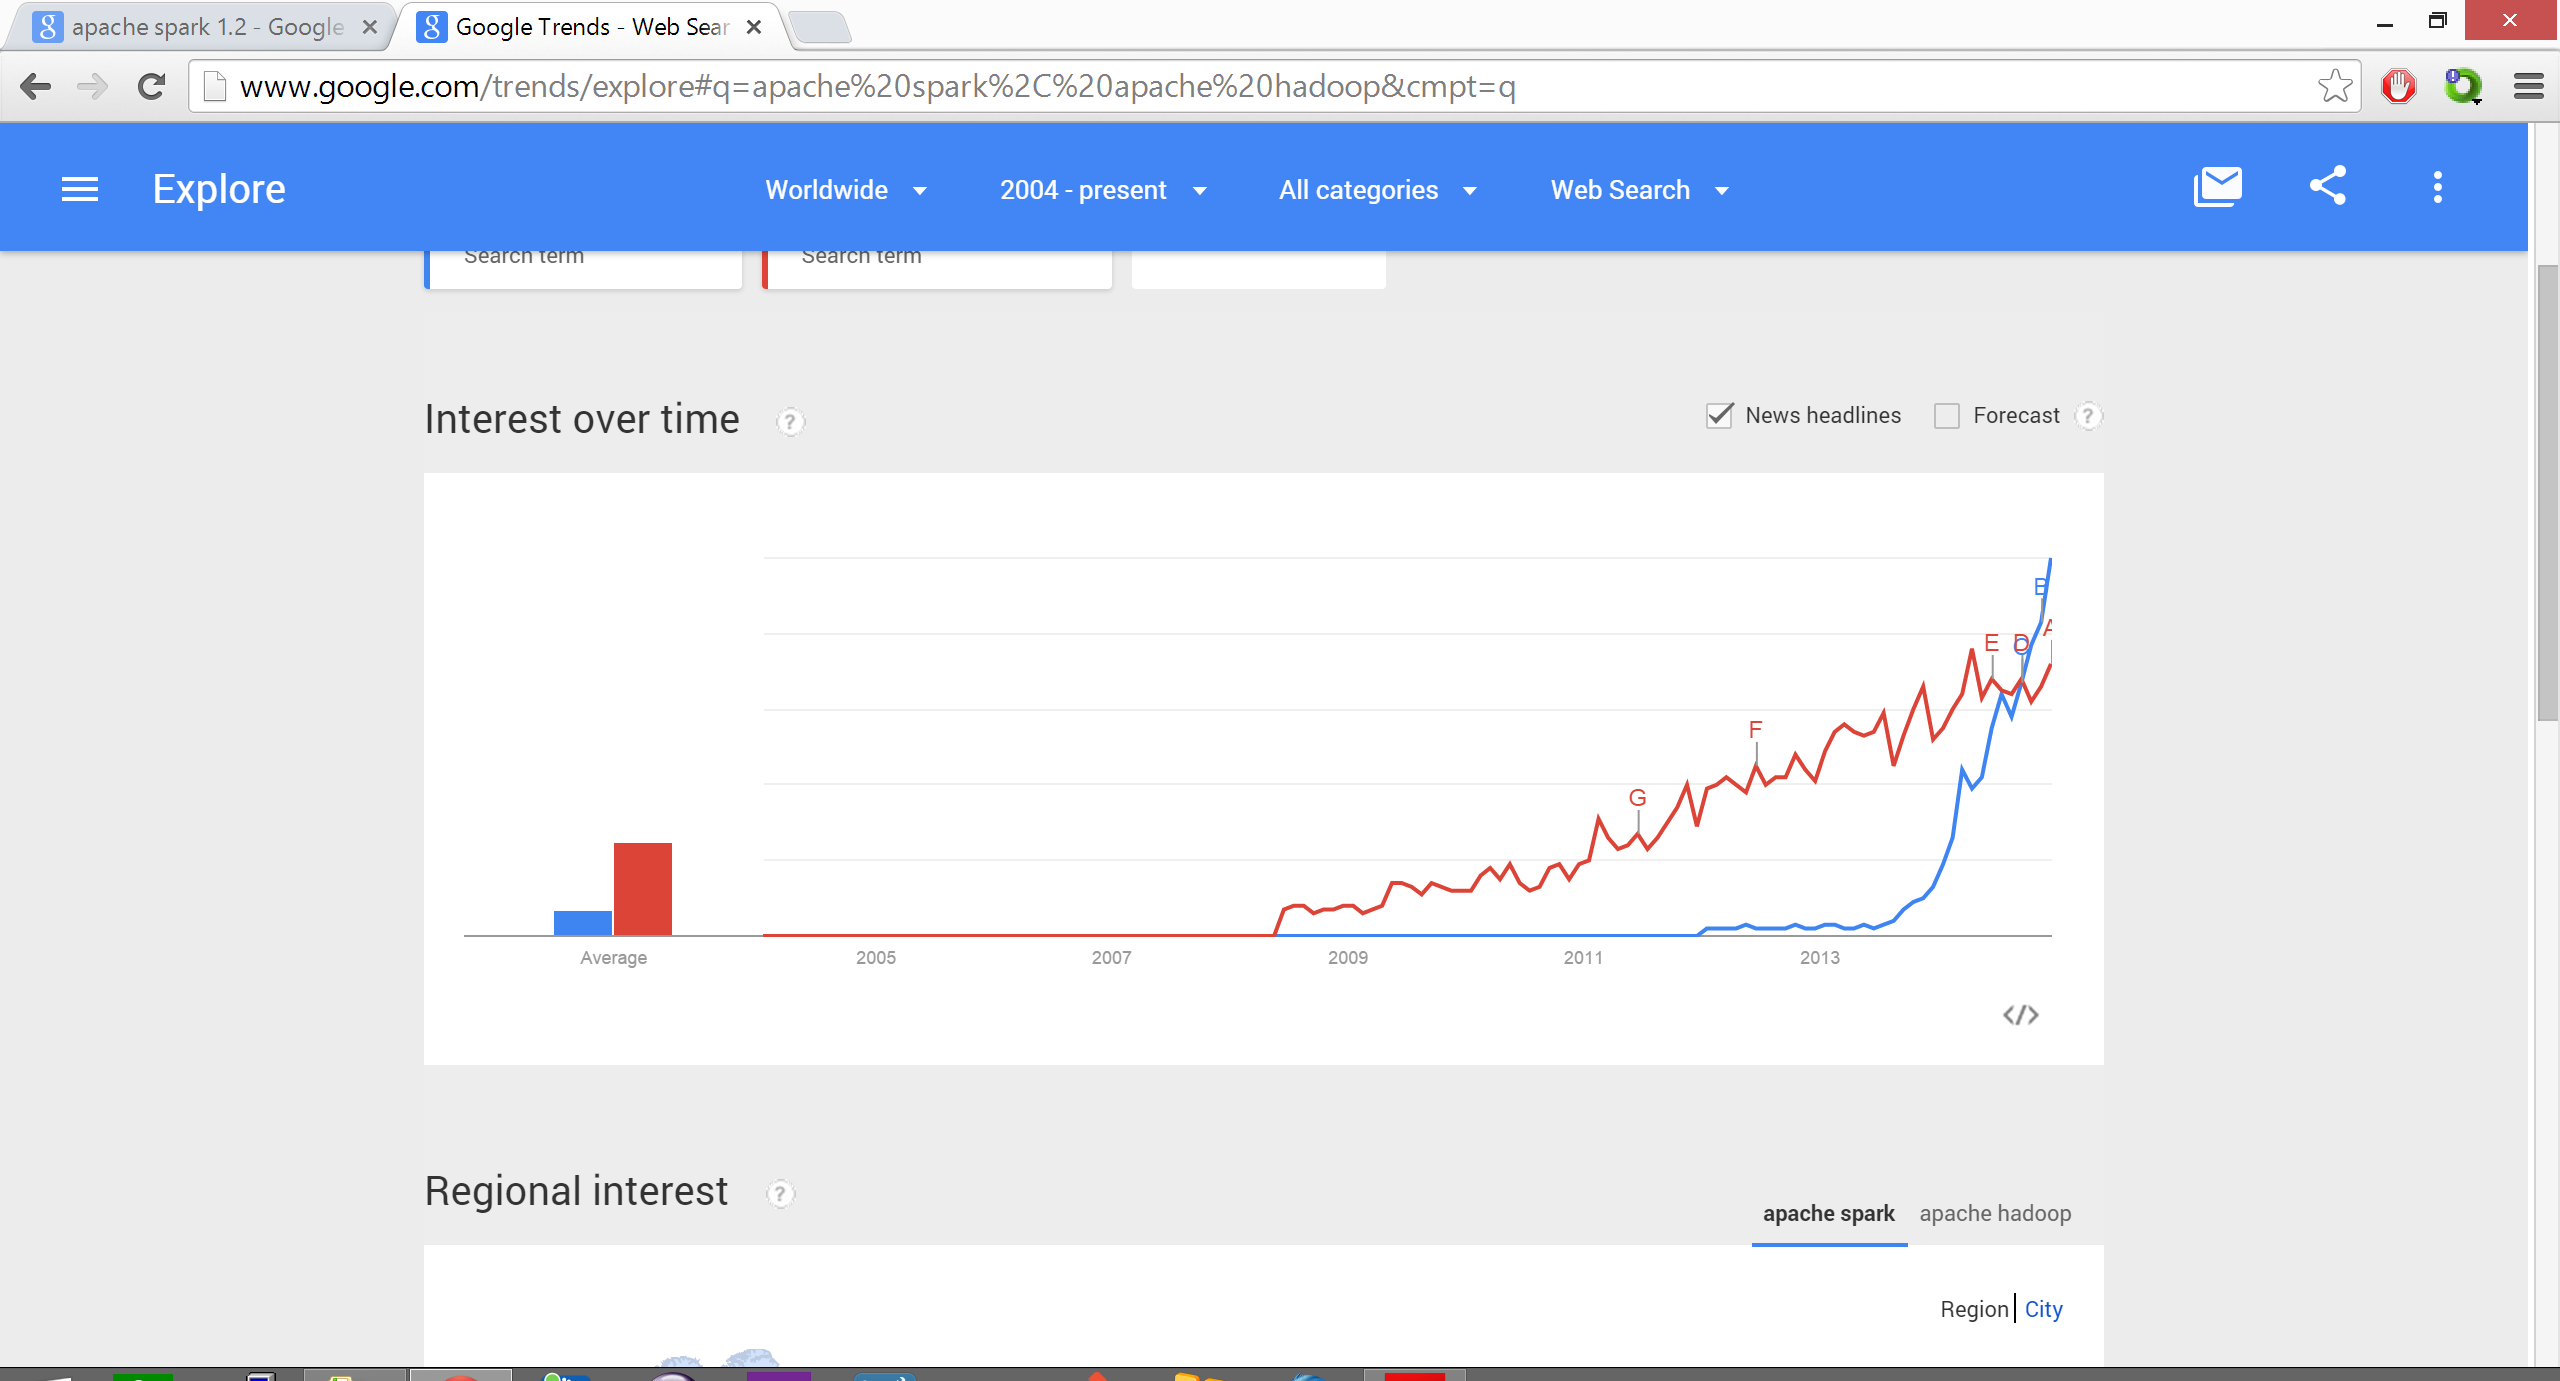
\includegraphics[scale=0.6]{bilder/trends_spark_vs_hadoop.PNG}
\caption[Google Trends]{Suchanfragen zu Spark (\textit{blau}) und Hadoop (\textit{rot}), Stand 24.03.2014 \cite{googletrends}}
\end{figure}

\section{Kontextabgrenzung}
Das Ziel dieser Arbeit ist es die grundlegenden Konzepte und Möglichkeiten von Apache Spark zu untersuchen und ausgewählte Aspekte im Rahmen konkreter Anwendungen zu betrachten.\\

Für ein tieferes Verständnis werden Installation, Cluster-Betrieb und die Modellierung und Implementation von Treiberprogrammen beispielhaft durchgeführt, dokumentiert und bewertet. Hierbei kommt Apache Spark in der Version 1.3.0 zum Einsatz.\\

Nur am Rande wird betrachtet:
\begin{itemize}
	\item Der Vergleich mit ähnlichen Produkten
	\item Die empirische Analyse des Skalierungsverhaltens
	\item Details zu Installation und Betrieb
\end{itemize}

Apache Spark ist überwiegend in der Programmiersprache Scala geschrieben. Die Beispiele in dieser Arbeit werden ebenfalls in Scala verfasst um
\begin{enumerate}
	\item einen einheitlichen Stil und Vergleichbarkeit zwischen Quellcode-Auszügen und eigenen Beispielen zu gewährleisten.
	\item Ausdrücke in kurzer, prägnanter Form darzustellen.
\end{enumerate}

\chapter{Vorstellung von Apache Spark}
Aus Sicht eines Nutzers ist Apache Spark eine API zum Zugriff auf Daten und deren Verarbeitung.\\

Diese API (wahlweise für die Programmiersprachen Scala, Java und Python verfügbar), kann im einfachsten Fall über eine eigene Spark Konsole mit \gls{repl}\footcite{Hail} verwendet werden.\\
Die Zählung von Wortvorkommen in einem Text - das "`Hello World"' der Big Data Szene - lässt sich dort mit zwei Befehlen realisieren (Listing 2.1).\\

\begin{lstlisting}[caption=Word Count in der Spark Konsole]
my_dollar ./spark-shell
[...]
     / __/__  ___ _____/ /__
    _\ \/ _ \/ _ `/ __/  '_/
   /___/ .__/\_,_/_/ /_/\_\   version 1.3.0
      /_/
Using Scala version 2.10.4 (OpenJDK 64-Bit Server VM, Java 1.7.0_75)
Type in expressions to have them evaluated.
[...]
scala> val text = sc.textFile("../Heinrich Heine - Der Ex-Lebendige")
[...]
scala> :paste
text.flatMap(line => line.split(" "))
.map(word => (word, 1))
.reduceByKey(_ + _)
.collect()
[...]
res0: Array[(String, Int)] = Array((Tyrann,,1), (im,2), (Doch,1) ...)

\end{lstlisting}


Aus Sicht eines Administrators oder Softwarearchitekten ist Apache Spark eine Applikation auf einem \gls{cluster}, die sich in der Anwendungsschicht befindet und charakteristische Anforderungen insbesondere an Lokalität des Storages und die Netzwerkperformance stellt.\\

Was das konkret bedeutet, welche Mechanismen und Konzepte dahinterstehen und in welchem Ökosystem von Anwendungen sich Apache Spark bewegt wird in den folgenden Abschnitten dieses Kapitels beleuchtet.

\section{Überblick}
Im Allgemeinen Fall läuft eine Spark-Anwendung auf drei Arten von Rechnern (s. Abb. \ref{figure:sparkdeployment}):

\begin{enumerate}
	\item \textbf{Clientknoten}\\
	Auf Nutzerseite greift die Anwendung auf die API eines lokalen Spark-Kontextes zu, der die Kontaktdaten eines Clustermanagers sowie verschiedene Konfigurationseinstellungen enthält. 
	
	\item \textbf{\gls{master}knoten}\\
	Der \gls{master}knoten betreibt den \textit{Clustermanager} läuft auf einem entfernten Rechner und ist der Einstiegspunkt in den \gls{cluster}. Hier werden Aufträge des Anwenders an die Arbeitsknoten verteilt und Ergebnisse eingesammelt und zurückgereicht.
	
	\item \textbf{\gls{worker}knoten}\\
	Die \gls{worker}knoten beherbergen die Spark \textit{Executors} und sind die ausführenden Elemente der Aktionen und Transformationen. Die \textit{Executors} können untereinander Zwischenergebnisse austauschen und melden ihre Ressourcenverfügbarkeit an den \textit{Clustermanager}.
\end{enumerate}

\begin{figure}[ht!]
	\centering
  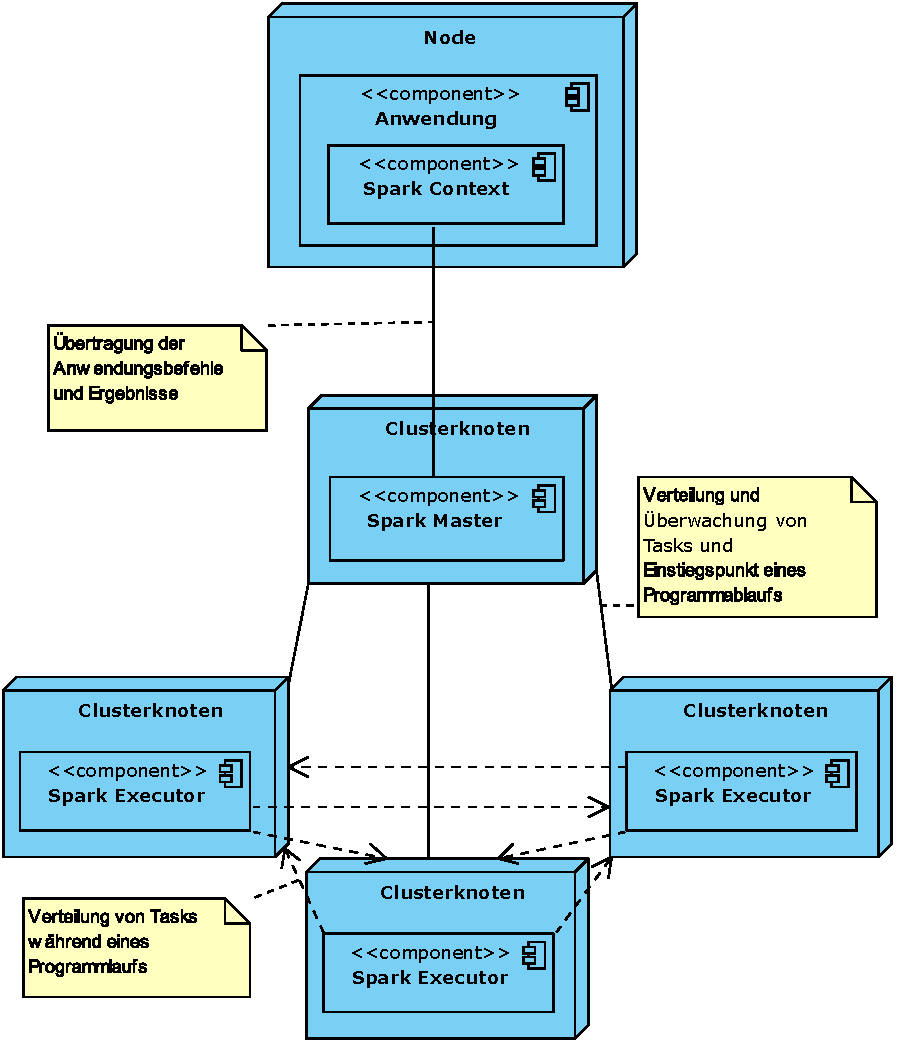
\includegraphics[pdf,scale=0.7]{sparkdeployment2}
	\caption{Verteilungsdiagramm einer typischen Sparkinstallation}
	\label{figure:sparkdeployment}
\end{figure}

Um die Architektur und Optimierungskonzepte eines verteilten Systems bewerten zu können ist es offensichtlich wichtig, welche Eigenschaften der unterliegenden Hardware angenommen werden.

Weil Spark explizit für den Betrieb innerhalb eines Hadoop/YARN \textcolor{red}{[VERWEIS auf Abschnitt Scheduling]} geeignet ist und YARN wiederum für den Betrieb auf einem \gls{cluster} auf Mittelklasse-Mehrzweckmaschinen (Commodity Hardware) optimiert ist\footcite{Mer14}, kann für Spark von einer vergleichbaren Hardwarekonfiguration ausgegangen werden.\\

Der Vergleich von drei aktuellen Rack Servern der 2000-Euro-Klasse (in der Grundausstattung) - hier als Mittelklasse-Geräte bezeichnet - liefert die folgenden Verhältnisse der wesentlichen Schnittstellen zueinander (Siehe Anhang~\ref{subsec:commodity_servers}).

\begin{table}[ht]
	\centering % used for centering table
	\begin{tabular}{c c c} % centered columns (4 columns)	
		\hline\hline %inserts double horizontal lines
		Netzwerk & Festspeicher & Arbeitsspeicher\\ [0.5ex] % inserts table
		%heading
		\hline % inserts single horizontal line
		0,125 GB/s & 1 GB/s & 17 GB/s \\ % inserting body of the table
		\hline %inserts single line
	\end{tabular}
	\caption{Theoretische Spitzenleistungen bei Mittelklasse-Servern} % title of Table
	\label{table:vgldurchsatz} % is used to refer this table in the text
\end{table}

Auf eine detaillierte Analyse des Zugriffsverhaltens wird im Rahmen dieser Arbeit verzichtet. Bei den folgenden Bewertungen der Kernkonzepte ist es wichtig sich die aus Tabelle \ref{table:vgldurchsatz} abgeleiteten Größenordnungen des Durchsatzes (\textit{D}) der verschiedenen Datenkanäle zu vergegenwärtigen:

\begin{equation*}
	D_{Netzwerk} < D_{Festspeicher} < D_{Arbeitsspeicher}
\end{equation*}

Für eine effiziente Verarbeitung von Daten ist es - ganz allgemein - also wünschenswert den größten Anteil des Datentransfers im Arbeitsspeicher zu haben, einen kleineren Anteil auf der Festplatte und einen noch kleineren Anteil auf Netzwerkverbindungen.\\

Es ist das oberste Ziel der folgenden Kernkonzepte von Apache Spark unter diesen Bedingungen die effiziente Verarbeitung \textit{großer Datenmengen}\footcite{Sam14} zu gewährleisten.\\

\section{Kernkonzepte}
Die universelle Einheit mit der ein Datenelement auf Spark repräsentiert wird ist ein sogenanntes \gls{rdd}\footcite{Mat12}.\\

Die gesamte operative Kern-API dreht sich um die Steuerung dieser Datenelemente. Insbesondere sind auch die in den Standardbibliotheken verfügbaren "`höheren"' APIs auf diesen \glspl{rdd} implementiert.
\glspl{rdd} sind damit die wichtigste Abstraktion des Applikationskerns.\\

In erster Näherung können \glspl{rdd} als eine Variante von \gls{dsm}\footcite{Nitzberg:1991:DSM:112827.112855} \cite{Mat12} verstanden werden, haben allerdings sehr charakteristische Einschränkungen und Erweiterungen, die im Folgenden erläutert werden.\\

\begin{figure}[ht!]
	\centering
  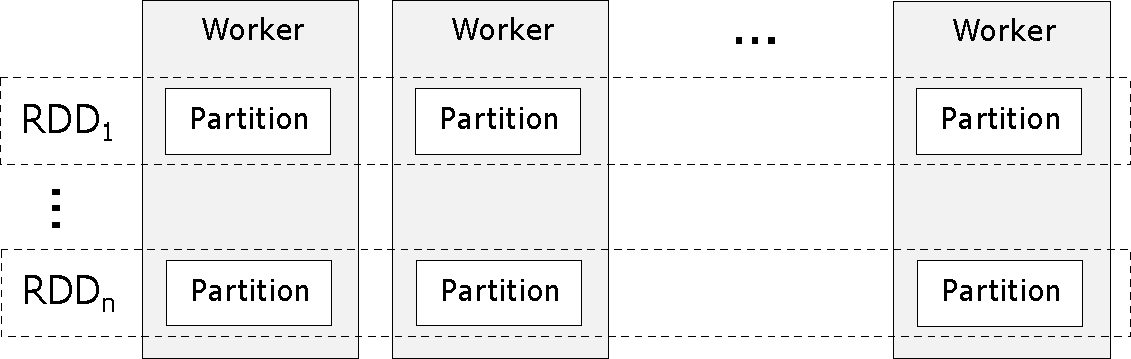
\includegraphics[pdf,scale=0.7]{RDDs1}
	\caption{Resilient Distributed Datasets aus Verteilungssicht}
	\label{figure:rdds1}
\end{figure}

\subsection{Nutzung von Arbeitsspeicher}

\subsection{Nutzung von persistentem Speicher}
\subsection{Nutzung von CPUs}
\subsection{Scheduling/Shuffling}
\subsection{Kern-API}
\paragraph{Transformationen}
\paragraph{Aktionen}

\section{Standardbibliotheken}
\textcolor{gray}{--- Warum ist Spark so einfach (und wo vielleicht nicht)? ---}\\
Die vier Standardbibliotheken erweitern die Kern-API für bestimmte, häufig genutzte Aufgaben aus Bereichen der Datenanalyse.\\

Die bedienten Bereiche sind
\begin{itemize}
	\item Deklaratives Abfragen auf strukturierten Datensätzen (\textit{Spark SQL})
	\item Maschinenlernverfahren (\textit{MLlib})
	\item Echtzeitbehandlung von eingehenden Daten (\textit{Streaming})
	\item Operationen auf Graph-Strukturen (\textit{GraphX})
\end{itemize}

\subsection{Dataframes/Spark SQL}
\subsection{MLlib}
\subsection{Streaming}
\subsection{GraphX}

\section{Betrieb und Security}

\section{Spark im Kontext von Parallelisierungspattern}
\textcolor{gray}{--- Buch: Algorithms and Parallel Computing ---}\\

\section{Entwicklergemeinschaft}
\textcolor{gray}{--- Herkunft, Apache Foundation, Entwicklungsphilosophien, Anzahl Entwickler, ... ---}\\

\section{Verwandte Produkte}
\textcolor{gray}{--- Ergänzende oder konkurrierende Produkte ---}\\
\subsection{YARN}
\subsection{Mesos}
\subsection{Flink}
\subsection{MPI}
\subsection{Kafka}
\subsection{HBase}
\subsection{Lustre}

\chapter{Entwicklung und Betrieb einer Beispielanwendung}

In diesem Kapitel wird die Entwicklung einer Anwendung für Spark und der Betrieb auf einem Cluster mit leistungsschwacher Hardware demonstriert und untersucht.

\section{Vorstellung der Beispielanwendung}

Als Demonstration der Anwendungsentwicklung und des Anwendungsbetriebes mit Spark soll ein Backend zur Nachrichtenanalyse implementiert werden.\\

Nachrichten sind in diesem Fall Tweets, die über die kostenlose Streaming-\gls{api}\footnote{https://dev.twitter.com/streaming/sitestreams, abgerufen am 06.06.2015} von Twitter\footnote{https://twitter.com, abgerufen am 06.06.2015} übertragen  und anschließend bewertet werden sollen.\\

Die Bewertung soll anhand inhaltlicher Ähnlichkeit mit aktuellen Diskussionen innerhalb der Mailingliste\footnote{user@spark.apache.org, abgerufen am 15.06.2015} von Sparkbenutzern erfolgen.\\

In Abbildung~\ref{figure:demo_app_usecase} wird der zugehörige Anwendungsfall dargestellt. Für die Beispielanwendung wird nur das Backend implementiert. Die grafische Benutzeroberfläche wird jedoch stellenweise erwähnt, um einen klaren Kontext zu setzen.\\

\begin{figure}[ht!]
	\centering
  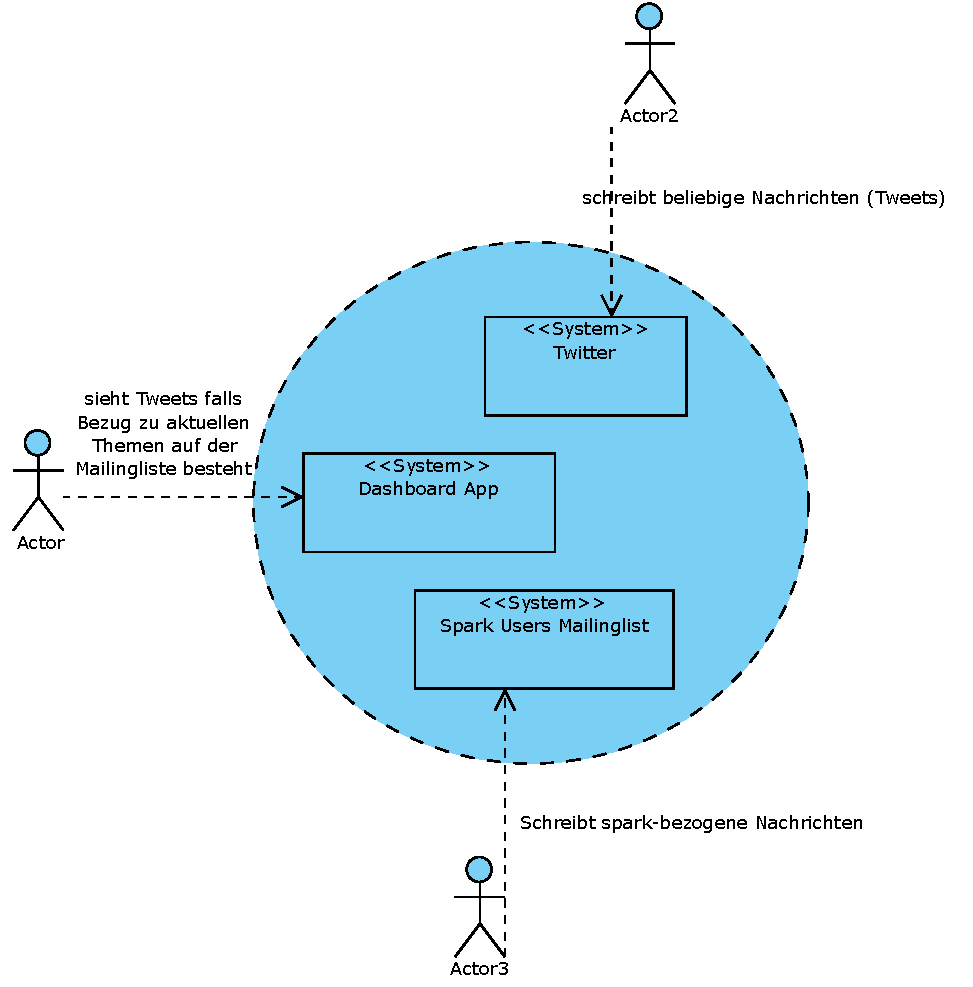
\includegraphics[width=0.9\textwidth]{demo_app_usecase.pdf}
	\caption{Anwendungsfalldiagramm der Demo-Applikation}
	\label{figure:demo_app_usecase}
\end{figure}

Die Analyse der Tweets soll in Quasi-Echtzeit erfolgen und direkt anschließend an eine Datensenke weitergereicht werden (dort wäre beispielsweise eine Messagequeue oder Datenbank zur Weiterleitung an eine grafische Benutzeroberfläche).\\

Bis zu zehn Sekunden Latenz vom Eingang der Nachricht bis zur Weiterleitung an die Senke seien hier als \textit{Quasi-Echtzeit} akzeptabel.\\

Als \textit{aktuelle Diskussionen} in der Mailingliste der Sparkbenutzer gelten solche, die innerhalb der letzten etwa 500 Nachrichten geführt wurden. Bei der Bewertung neuer Nachrichten gibt es hier keine Echtzeit-Anforderung. Die Neubewertung bei Eintreffen neuer Nachrichten - höchstens etwa alle 30 Minuten - soll genügen.\\

\section{Hardwareumgebung}

Als Versuchsumgebung dient ein \gls{cluster} aus vier identischen \gls{worker}n und einem speziellen \gls{master}knoten (Abb. \ref{figure:versuchsaufbau}).

\begin{figure}[h]
	\centering
  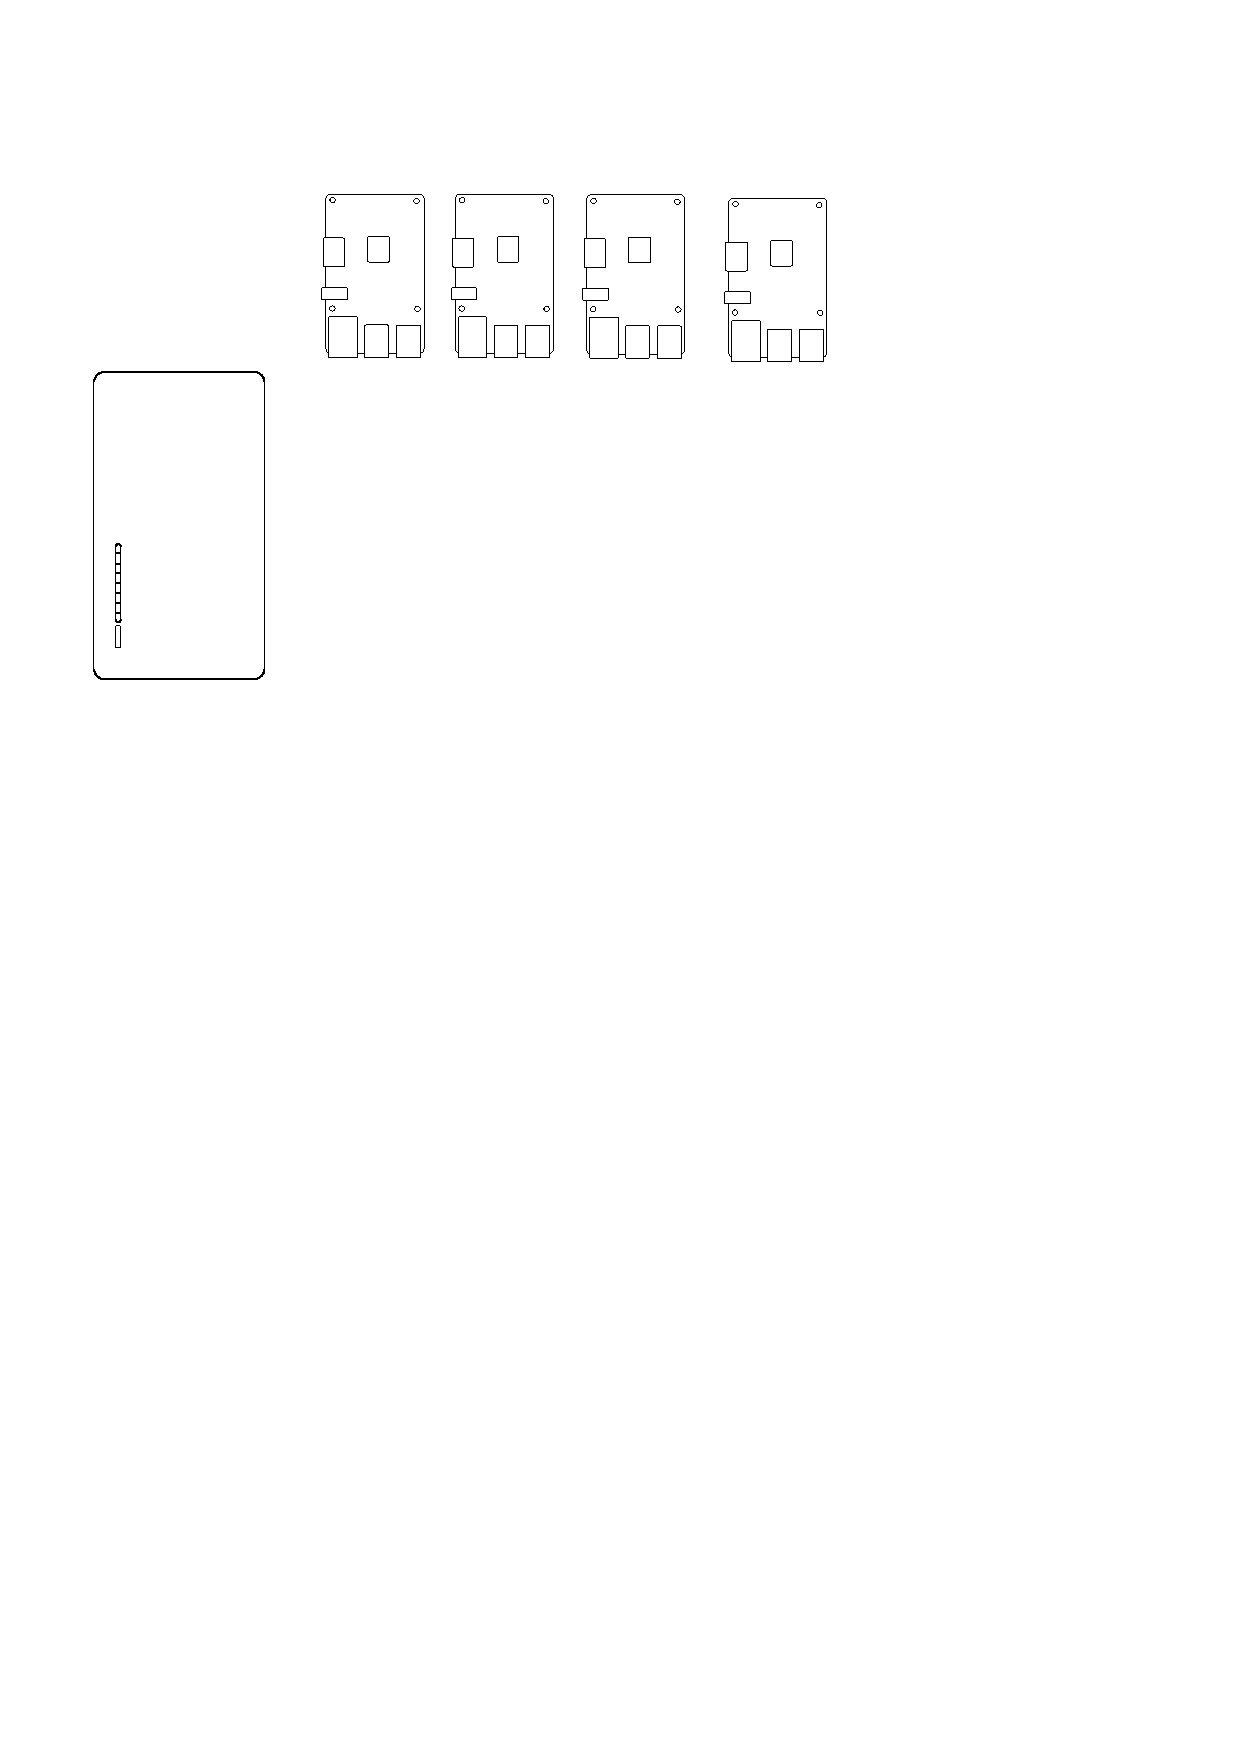
\includegraphics[width=0.7\textwidth]{versuchsaufbau.pdf}
	\caption{Hardwareumgebung des Programms zur Tweetanalyse}
	\label{figure:versuchsaufbau}
\end{figure}

Dieser Cluster besteht aus ausschließlich aus leistungsschwacher Hardware. Mit \textit{leistungsschwach} sind Geräte gemeint, deren Leistungsfähigkeit noch deutlich unter aktueller sogenannter \textit{Commodity Hardware} liegt (Vgl. Anhang~\ref{subsec:commodity_servers}).\\

Konkret kommen die folgenden Geräte zum Einsatz:

\paragraph{Worker}
Rasperry Pi 2
\begin{itemize}
	\item CPU: 900MHz Quad-Core ARM Cortex A7
	\item RAM: 1GB SDRAM
	\item Ethernet: 100MBit/s
	\item Festspeicher: SDHC Class 4 Speicherkarte 16GB
\end{itemize}
Als Betriebssystem wird das Debian-Derivat Raspbian\cite{raspbian} 32-Bit genutzt.

\paragraph{Master}
Dell d420
\begin{itemize}
	\item CPU: 1,2 GHz Core2 Duo U2500
	\item RAM: 2GB DDR2 SDRAM
	\item Ethernet: 100MBit/s
	\item Festspeicher: 60GB 4200RPM Hard Drive
\end{itemize}
Als Betriebssystem wird Ubuntu (\cite{ubuntu}) 14.04 32-Bit genutzt.

\paragraph{Netzwerk}
Die Rechner sind mit \gls{rj45} über einen TP-Link TL-SF1008D Switch mit theoretischem maximalem Durchsatz von 100MBit/s vernetzt.

Als Basisdaten für die Leistungsfähigkeit der eingesetzten Hardware werden zusätzliche Tests durchgeführt, deren Ergebnisse in Tabelle \ref{table:network}, Tabelle \ref{table:master_harddrive} und Tabelle \ref{table:master_harddrive} aufgeführt sind.

\begin{table}[ht]
	\centering % used for centering table
	\begin{tabular}{c c c c} % centered columns (4 columns)
	\hline\hline %inserts double horizontal lines
	Worker $\rightarrow$ Worker & Worker $\rightarrow$ Master \\ [0.5ex] % inserts table
	%heading
	\hline % inserts single horizontal line
	94,4 MBit/s & 94,4 MBit/s\\ [1ex] 
	\hline %inserts single line
	\end{tabular}
	\caption{Maximaler Netzwerkdurchsatz{\protect\footnotemark}} % title of Table
	\label{table:network} % is used to refer this table in the text
\end{table}
\footnotetext{Gemessen mit \lstinline|iperf|. Siehe Anhang Listing~\ref{lst:measure_network}}

\paragraph{Festspeicher}

\begin{table}[ht]
	\centering % used for centering table
	\begin{tabular}{c c c c} % centered columns (4 columns)
	\hline\hline %inserts double horizontal lines
	Operation & Blockgröße (MB) & Durchsatz (MB/s) \\ [0.5ex] % inserts table
	%heading
	\hline % inserts single horizontal line
	Lesen & 1 & 17,2 \\ 
	Lesen & 16 & 22,1 \\
	Lesen & 64 & 31,8 \\
	Lesen & 512 & 31,2 \\
	Schreiben & 1 & 5,0 \\
	Schreiben & 16 & 17,2 \\
	Schreiben & 64 & 26,1 \\
	Schreiben & 512 & 25,8 \\[1ex] 
	\hline %inserts single line
	\end{tabular}
	\caption{Festspeicher Lese-/Schreibdurchsatz dell01 (Master){\protect\footnotemark}} % title of Table
	\label{table:master_harddrive} % is used to refer this table in the text
\end{table}
\footnotetext{Gemessen mit \lstinline|dd|. Siehe Anhang Listing~\ref{lst:measure_harddrive}}

\begin{table}[ht]
	\centering % used for centering table
	\begin{tabular}{c c c c} % centered columns (4 columns)
	\hline\hline %inserts double horizontal lines
	Operation & Blockgröße (MB) & Durchsatz (MB/s) \\ [0.5ex] % inserts table
	%heading
	\hline % inserts single horizontal line
	Lesen & 1 & 66,4 \\ 
	Lesen & 16 & 78,1 \\
	Lesen & 64 & 42,0 \\
	Lesen & 512 & 9,2 \\
	Schreiben & 1 & 17,9 \\ 
	Schreiben & 16 & 18,4 \\
	Schreiben & 64 & 18,4 \\
	Schreiben & 512 & 18,4 \\[1ex] 
	\hline %inserts single line
	\end{tabular}
	\caption{Festspeicher Lese-/Schreibdurchsatz pi00 (Worker)} % title of Table
	\label{table:worker_harddrive} % is used to refer this table in the text
\end{table}

\section{Lösungsskizze}
\paragraph{Wahl des Dateisystems}

Für diesen Versuch wird das Hadoop Dateisystem \textit{HDFS} in der Version 2.7.0 gewählt.\\

Dieses Dateisystem gewährleistet die verteilte Speicherung von Blöcken auf dem Cluster und bietet Konfigurationsmöglichkeiten die direkten Einfluss auf die Performance von Spark haben.\\

Zu diesen Konfigurationsmöglichkeiten gehören insbesondere die Größe der Blöcke und die Anzahl der Replikate eines Blockes.\\

\paragraph{Wahl des Cluster-Managers}

Spark läuft in diesem Versuch als alleinige Computeanwendung auf dem Cluster. Es ist also nicht nötig Konkurrenz um Ressourcen zu berücksichtigen. Für diesen Versuch wird daher der Standalone Clustermanager gewählt.\\

\paragraph{Architekturübersicht}\\
\\

Die Architektur der Beispielanwendung teilt die Anwendungslogik in drei Schichten auf. \\
In einer Schicht findet die Verarbeitung eingehender Emails statt und es werden die Relevanz der Begriffe bewertet (\textit{Batch Layer}).
In einer zweiten Schicht werden die Tweets aus einem Datenstrom eingelesen und deren Relevanz anhand der Bewertungen aus der ersten Schicht bewertet (\textit{Streaming Layer}).\\
In der dritten Schicht werden die als relevant eingestuften Emails in einer grafischen Oberfläche dem Benutzer zur Verfügung gestellt (\textit{Presentation Layer}). Diese Schicht gehört nicht zum Spark-Backend und wird für diese Demonstation nicht implementiert.

\begin{figure}[ht!]
	\centering
  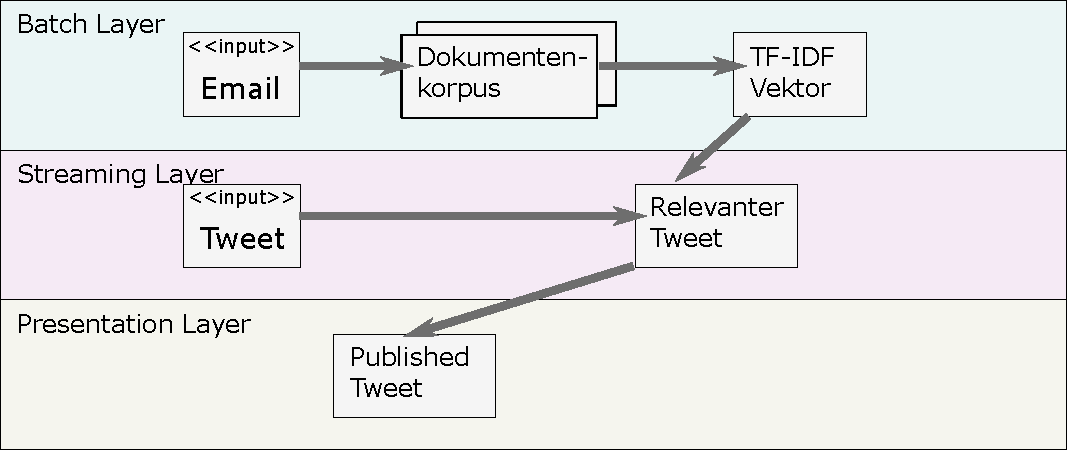
\includegraphics[scale=0.7]{data_centric_layers.pdf}
	\caption{Datenzentrierte Sicht auf die Komponenten}
	\label{figure:data_centric_layers}
\end{figure}

\paragraph{Batch Layer}\\
\\

In dieser Schicht wird die Verarbeitung von Emails aus der Spark-User-Mailingliste zu einem Modell von relevanten Wörtern geleistet.\\

Dazu werden eingehende Emails zunächst archiviert und anschließend mithilfe des Korpus aller bisher archivierten Emails und einer Untermenge von \textit{n} zuletzt empfangenen Emails eine Bewertung der vorkommenden Wörtern vorgenommen.\\

Diese Bewertung soll das Maß für die Relevanz eines Wortes in der betrachteten Menge der letzten \textit{n} Emails sein. Um das zu erreichen, wird in mehreren Schritten ein TF-IDF Vektor über die Wörter dieser Nachrichten erzeugt.\\

\begin{figure}[ht!]
	\centering
  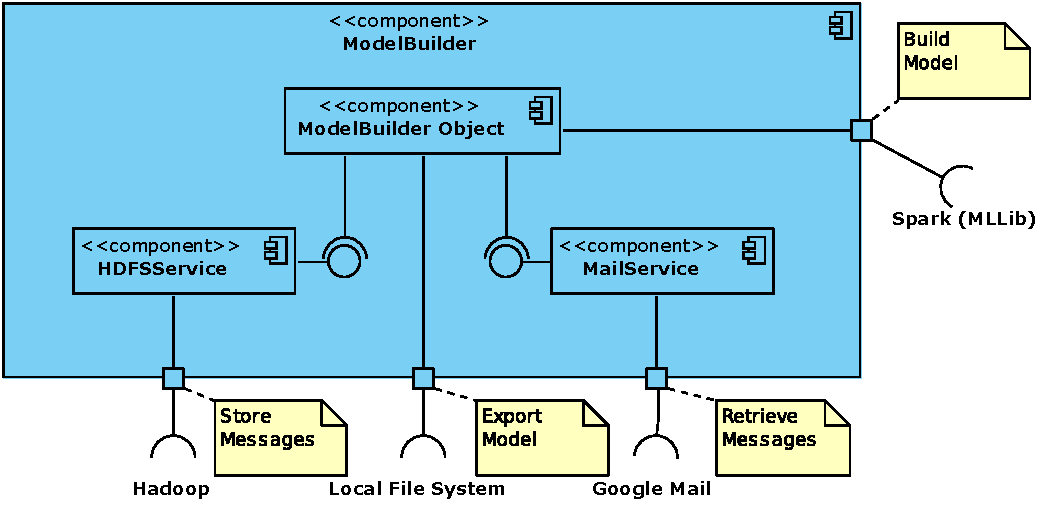
\includegraphics[width=\textwidth]{batch_layer.pdf}
	\caption{Innenansicht der Batch-Layer Komponente}
	\label{figure:demo_app_batchlayer}
\end{figure}

TF-IDF steht für \textit{Term Frequency - Inverse Document Frequency} (\cite{SparckJones:1988:SIT:106765.106782}). Dieses Verfahren bewertet die Relevanz eines Wortes für einen Text nach der Häufigkeit dieses Wortes in dem Text (\textit{Term Frequency}). Die Bewertung eines Wortes wird jedoch abgeschwächt je häufiger es in einem Textkorpus vorkommt (\textit{Inverse Document Frequency}).\\

Eine Implementation dieses Verfahrens ist in der Spark Standardbibliothek \textit{MLLib} in dem Bereich \textit{Feature Extraction} verfügbar\footnote{https://github.com/apache/spark/tree/branch-1.3/mllib/src/main/scala/org/apache/spark/mllib/feature, abgerufen am 04.06.2015}.\\

In diesem Anwendungsfall gilt:
\begin{itemize}
\item Email-Bodies\footnote{Textbereich einer Email} werden jeweils als Dokumente verarbeitet
\item Das Archiv aller Email-Bodies ist der Textkorpus
\end{itemize}

Die Prozedur beginnt mit dem Definieren eines \gls{rdd} aus der Textdatei aller Emailnachrichten (\lstinline|textfile|).\\

\begin{lstlisting}
val documents: RDD[Seq[String]] = sc.textFile(textFile)
  .map(_.toLowerCase)
  .map(_.split(" ").filter(_.length > 2).toSeq)
\end{lstlisting}

Diese Textdatei wird durch \lstinline|ModelBuilder| regelmäßig ergänzt sofern der IMAP-Client neue Nachrichten aus der Mailingliste empfangen hat.\\

Anschließend werden die Elemente des \gls{rdd} \lstinline|documents| von einer Sequenz von Wörtern auf einen Vektor der Worthäufigkeiten abgebildet:

\begin{lstlisting}
val tf: RDD[Vector] = hashingTF.transform(documents)
\end{lstlisting}

Mit diesem RDD von Vektoren der Worthäufigkeiten wird nun ein Modell (\lstinline|IDF|, \textit{Inverse Document Frequency}) gebildet, dass die inversen Worthäufigkeiten berechnet. Dazu für jedes vorkommende Wort die Anzahl aller Dokumente ermittelt in denen es vorkommt.\\

Dieses Modell wird dann genutzt um die bereits berechneten Wortvorkommen pro Dokument anzupassen (\lstinline|idf.transform(tf)|). Es entstehen die TF-IDF Vektoren:

\begin{lstlisting}
val idf = new IDF().fit(tf)
val tfidf: RDD[Vector] = idf.transform(tf)
\end{lstlisting}

Der Relevanzvektor wird anschließend durch Aufsummieren der TF-IDF in der gewünschten Fenstergröße berechnet. Die Fenstergröße entspricht dem Bereich dessen spezifische Wörter in der Streaming Layer für das Scoring der Tweets benutzt werden sollen.

\begin{lstlisting}
val relevanceVector = tfidf
  .take(docWindowSize)
  .reduce((vector1, vector2) =>
    addSparseVectors(vector1.asInstanceOf[SparseVector], 
		vector2.asInstanceOf[SparseVector]))
\end{lstlisting}

\paragraph{Streaming Layer}\\
\\

In dieser Schicht werden die Nachrichten aus dem Twitter-Datenstrom bewertet und gefiltert.\\

Dazu wird über die Spark-Komponente \textit{TwitterUtils}\footnote{TwitterUtils sind Teil der Spark-Standardbibliothek org.apache.spark.streaming.twitter} eine Verbindung über HTTP zu einem Twitter-Endpunkt aufgebaut\footnote{https://dev.twitter.com/streaming/overview/connecting, abgerufen am 01.06.2015}. Über diese Verbindung werden - bei unpriveligiertem Zugriff - etwa 40 Tweets pro Sekunde über einen dauerhaften Datenstrom zur Verfügung gestellt (siehe Abb.~\ref{figure:realtime_dashboard_stats}).\\

\begin{figure}[ht!]
	\centering
  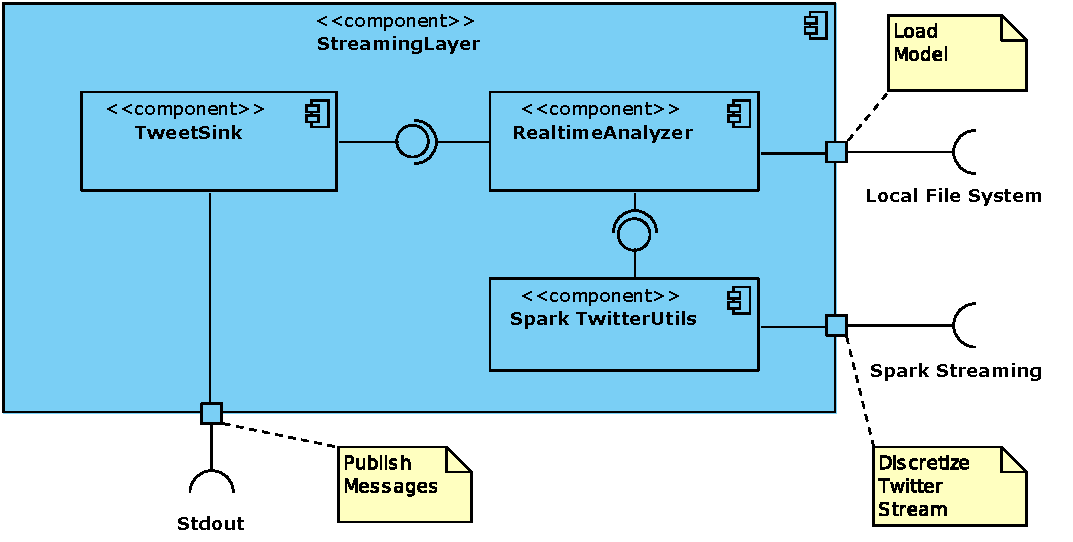
\includegraphics[width=\textwidth]{streaming_layer.pdf}
	\caption{Innenansicht der Streaming-Layer Komponente}
	\label{figure:demo_app_streaminglayer}
\end{figure}

In der Komponente RealtimeAnalyzer wurden vor dem Start des Datenstroms Funktionen zur Bewertung einzelner Tweets registriert.\\

Die Funktion \lstinline|ScoreTweets| zur Bewertung einzelner Tweets

\[\lstinline|ScoreTweets|: Tweets \longrightarrow \rm I\!R \times Tweets\]
\[tweet \mapsto (score, tweet)\]

wird dabei wie in Listing \ref{lst:tweet_score} dargestellt implementiert:

\begin{lstlisting}[language=Scala,caption={Bewertung von Tweets},label={lst:tweet_score}]
// Split text string into single words
val splitTweets = {
  stream.map(status =>
    (status.getText.split(" "), status)
  )
}

// calculate score for each word, then sum and normalize the scores
val scoredTweets = {
  splitTweets.map(splitTweet => {
    (splitTweet._1.map(word =>
      broadcastScores.value.apply(
         hashingTF.indexOf(word.toLowerCase
           .replaceAll("[^a-zA-Z0-9]", " ")))
     ).sum./(splitTweet._2.getText.split(" ").length),
      splitTweet._2
      )}
  )
}
\end{lstlisting}

Folgendes geschieht Folgendes:
\begin{enumerate}
	\item Extrahieren des Textinhaltes (Metadaten werden ignoriert)
	\item Zerlegen des Textes in einzelne Wörter
	\item Normalisieren der Wörter durch Umwandeln in Kleinbuchstaben und Entfernen von Sonderzeichen
	\item Index der einzelnen Wörter im TF-IDF-Vektor berechnen und dem eingetragenen Score zuweisen (\textit{Map})
	\item Scores aller Wörter eines Tweets summieren (\textit{Reduce})
	\item Normalisieren des Scores per Division durch die Anzahl aller Wörter des Tweets
	\item Rückgabe des Tupels \textit{(Score, Status)}
\end{enumerate}

Anschließend werden die erzeugten Tupel nach der Größe des erreichten Scores gefiltert und die verbleibenden Status-Texte an den TweetSink weitergegeben.\\

\begin{figure}[ht!]
	\centering
  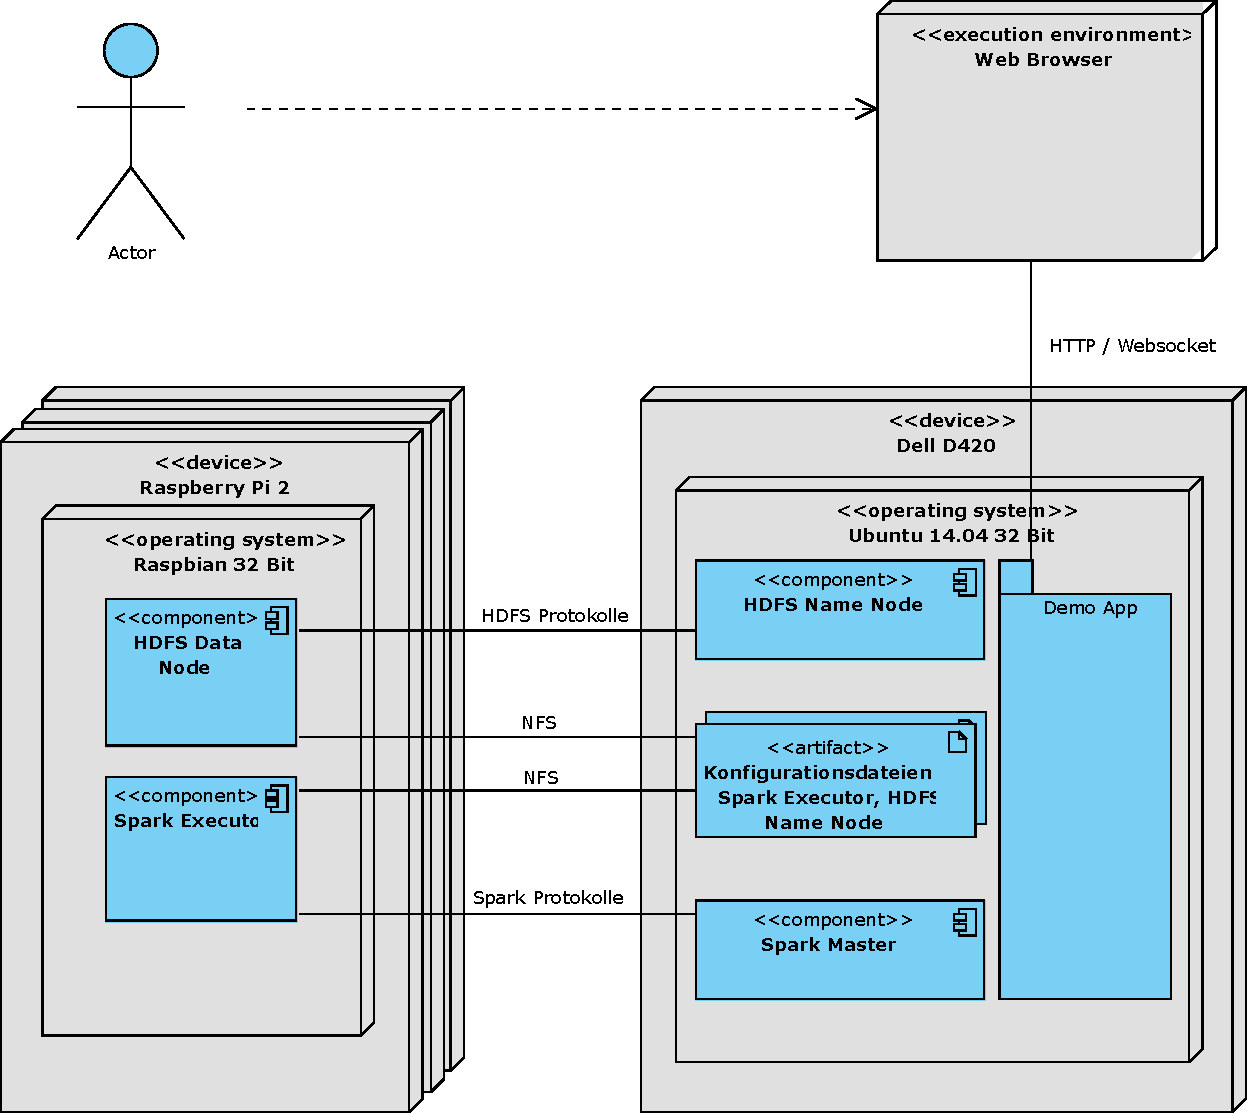
\includegraphics[width=0.9\textwidth]{demo_app_deployment.pdf}
	\caption{Verteilungssicht auf die Demo App}
	\label{figure:demo_app_verteilung}
\end{figure}


\begin{figure}[ht!]
	\centering
  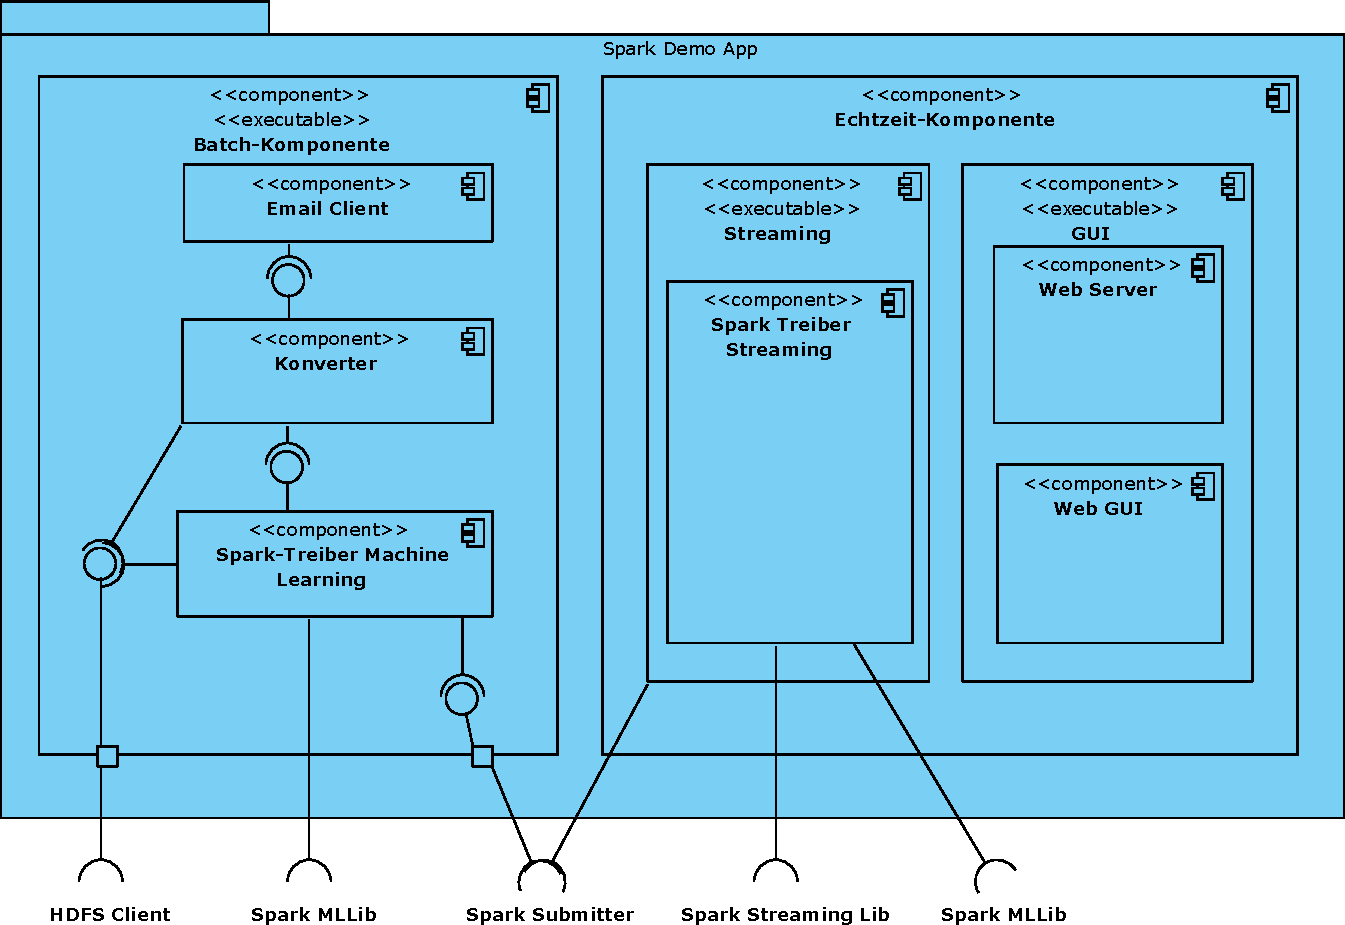
\includegraphics[width=0.9\textwidth]{demo_app_components.pdf}
	\caption{Komponentendiagramm des Demo App Packages}
	\label{figure:demo_app_komponenten}
\end{figure}

\section{Hinweise zur Entwicklung}
Die Komponenten werden in jeweils eigenen Projekten entwickelt, die sich einzeln auf dem Cluster deployen lassen. Das hat den Vorteil, dass eine einfache Continuous Deployment Pipeline (Abb.~\ref{figure:cd_pipeline}) eingesetzt werden kann, die Änderungen an den jeweiligen Projekten automatisiert auf dem Cluster deployt und so schnellstmögliches Feedback ermöglicht, sowie eine stets lauffähige Codebasis begünstigt.\\

\begin{figure}[ht!]
	\centering
  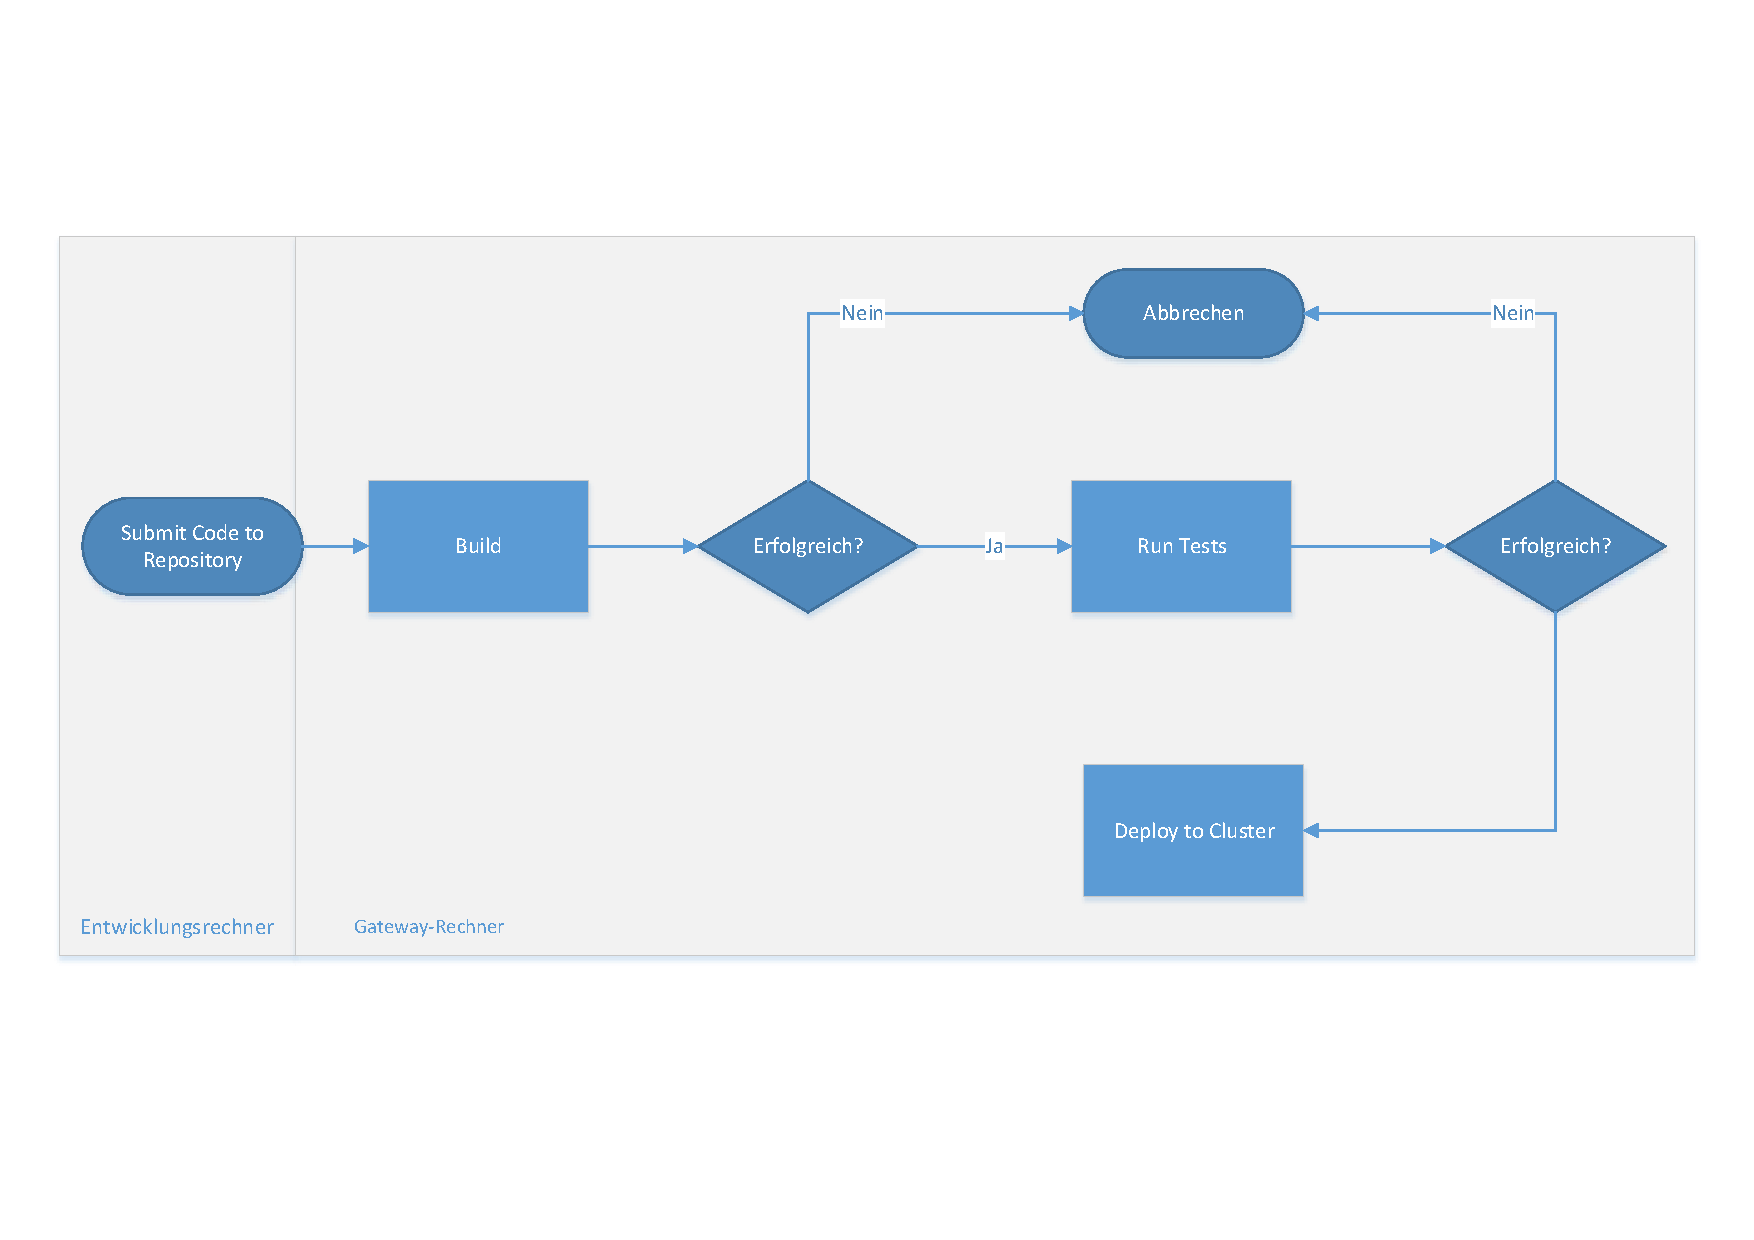
\includegraphics[width=0.9\textwidth]{Pipeline.pdf}
	\caption{Einfache Continuous Deployment Pipeline}
	\label{figure:cd_pipeline}
\end{figure}

Diese Pipeline ist durch ein \textit{post-receive}-Skript in den jeweiligen Repositories der Komponenten auf dem Gateway-Rechner realisiert (Beispiel im Anhang~\ref{subsec:pipeline}).\\


\section{Ergebnisse und Bewertung}

Zur Beurteilung des Laufzeitverhaltens wird die Anwendung in verschiedenen Konfigurationen des Raspberry-Pi-Clusters gestartet. Dabei wird jeweils das Verhalten der einzelnen Komponenten und des gesamten Systems erfasst und zur späteren Auswertung gespeichert.\\

Die zur Laufzeit erfassten Daten sind
\begin{enumerate}
	\item Systemgrößen auf jedem aktiven Knoten (1 Messpunkt pro Sekunde)
	\subitem CPU Nutzung (User, Idle, System, ...)
	\subitem IO Festplatte (Lesen, Schreiben)
	\subitem Swap (Benutzt, Frei)
	\subitem Speicher (Benutzt, Frei, Cached, ...)
	\subitem IO Netzwerk (Gesendet, Empfangen)
	\item Sparkspezifische Größen (1 Messpunkt alle zwei Sekunden)
	\subitem genutzte Cores
	\subitem aktive Stages
	\subitem parallele Receiver (bei Streaming)
	\subitem u.a.\footnote{Bei den sparkspezifischen Messgrößen gibt es viele weitere, die nicht in die Auswertungen einbezogen werden.}
\end{enumerate}

Als Konfigurationsparameter für die Testläufe werden verwendet
\begin{enumerate}
	\item die Blockgröße des Hadoop-Dateisystems HDFS (32MB, 64MB, 128MB)
	\item der Replikationsfaktor der Blöcke auf HDFS (1, 2, 3, 4)
	\item die Anzahl der Worker (1, 2, 4)
\end{enumerate}

Um eine Vergleichbarkeit der Testläufe untereinander zu erreichen werden folgende Größen festgelegt:
\begin{enumerate}
	\item Größe des Textkorpus: 1,5 GB
	\item Fenstergröße des TF-IDF Vektors: 500 Nachrichten
	\item Erlaubte Cores Pro Executor: 4
	\item Erlaubter Arbeitsspeicher pro Executor: 384 MB
	\item Zeitintervall für die Diskretisierung des Datenstroms (Streaming-Komponente): 5 Sekunden
\end{enumerate}

Die \textbf{Größe des Textkorpus} ergibt sich aus der Überlegung eine Datei zu Verarbeiten, die größer als der Arbeitsspeicher eines einzelnen Workers ist, theoretisch aber noch in den geteilten Speicher von vier Executor-Prozessen passt.\\

Die \textbf{Fenstergröße des TF-IDF Vektors} ist willkürlich gewählt. Der Wert 500 entspricht der Anzahl von Email-Nachrichten aus der Spark-User-Mailingliste.\\

Die erlaubten \textbf{Cores pro Executor} entsprechen genau den Verfügbaren Cores auf einem Worker. Damit ist eine volle Ausnutzung der verfügbaren Rechenleistung gewährleistet.\\

Der erlaubte \textbf{Arbeitsspeicher von 384MB pro Executor} lässt bei 1000MB Gesamtspeicher pro Knoten noch Spielraum für das Betriebssystem, den Worker-Prozess und insbesondere den HDFS Data Node für Caching von Dateiblöcken.\\

Das \textbf{Zeitintervall für die Diskretisierung des Datenstroms} richtet sich nach einem Wert, der für den behandelten Anwendungsfall noch als Echtzeit gelten kann.
Ein höherer Wert würde den notwendigen Puffer erhöhen und vermutlich die Verarbeitungszeit pro Datenelement verringern. Ein niedrigerer Wert würde vermutlich den nötigen Puffer verringern und die relative Verarbeitungszeit eines Datenelementes erhöhen. In der folgenden Analyse der Laufzeitverhaltens wird jedoch deutlich, dass der tatsächliche Wert weitgehend unkritisch für die Stabilität der Komponente ist.\\

Um die Testläufe unter möglichst kontrollierten Bedingungen zu starten, wurde bei jeder Änderung der Konfigurationsparameter das Hadoop-Dateisystem formatiert und der Spark-Cluster zurückgesetzt (inklusive Terminierung und Neustart aller zugehörigen Prozesse).

\subsection{Batch-Komponente}

Die Laufzeitmessung beginnt mit dem Start der ersten Aktion auf einem \gls{RDD} und endet mit der Rückgabe des Relevanzvektors.
Weil die Initialisierung erst zu diesem Zeitpunkt erfolgt, wird der gesamte Prozess von der Kontaktaufnahme zum Cluster und Übermittlung der Tasks bis zur Rückgabe des Ergebnisses gemessen (siehe Listing~\ref{lst:modelbuilder_measuring}).\\

\begin{lstlisting}[language=Scala,caption={Laufzeitmessung},label={lst:modelbuilder_measuring}]
    val documents: RDD[Seq[String]] = sc.textFile(textFile)
      .map(_.toLowerCase)                                // stage 0
      .map(_.split(" ").filter(_.length > 2).toSeq)      // stage 0
    val hashingTF = new HashingTF(1 << 20)
    val tf: RDD[Vector] = hashingTF.transform(documents) // stage 0
    tf.cache() // keep the tf cached because it will be used twice
		
    val beginFeatureExtraction = System.currentTimeMillis()

    val idf = new IDF().fit(tf)                          // stage 0/1
    val tfidf: RDD[Vector] = idf.transform(tf)           // stage 2

    val relevanceVector = tfidf
      .take(docWindowSize)                               // stage 2
      .reduce((vector1, vector2) =>
        addSparseVectors(vector1.asInstanceOf[SparseVector], 
				vector2.asInstanceOf[SparseVector])
      ) // end stage 2, execution ends here

    val finishFeatureExtraction = System.currentTimeMillis()
\end{lstlisting}

Die Zeilen 1-6 in Listing~\ref{lst:modelbuilder_measuring} wurden in die Darstellung aufgenommen, um die Lineage vollständig darzustellen.\\

Der übrige Teil der Anwendung - insbesondere das Abrufen und Prozessieren neu eingegangener Emails - wird nicht berücksichtigt. Bei einem laufenden System sind die dort entstehenden Lasten so gering, dass kein Bedarf für Skalierung besteht.

Tabelle~\ref{table:scaling} zeigt die Laufzeiten der Modelbuilderkomponente bei verschiedenen Konfigurationseinstellungen des Clusters.

\begin{table}[ht]
	\centering % used for centering table
	\begin{tabular}{c c c c} % centered columns (4 columns)
	\hline\hline %inserts double horizontal lines
	Anzahl Worker & Replikationslevel & HDFS Blockgröße (MB) & Laufzeit (Sekunden) \\ [0.5ex] % inserts table
	%heading
	\hline % inserts single horizontal line
	1 & 1 & 32 & 697 \\ % inserting body of the table
	1 & 1 & 64 & 750 \\
	1 & 1 & 128 & 850 (*)\\
	2 & 2 & 32 & 366 \\
	2 & 2 & 64 & 448 \\
	2 & 2 & 128 & 615 \\
	4 & 3 & 32 & 210 \\
	4 & 4 & 32 & 209 (*)\\
	4 & 2 & 64 & 301 \\
	4 & 3 & 64 & 359 \\
	4 & 2 & 128 & 432 \\
	4 & 3 & 128 & 433 \\ [1ex] 
	\hline %inserts single line
	\end{tabular}
	\caption{Skalierungsverhalten des ModelBuilders - mit * sind jeweils die schnellste und langsamste Konfiguration markiert} % title of Table
	\label{table:scaling} % is used to refer this table in the text
\end{table}

Einen besonderen Einfluss auf die Laufzeit hat offenbar die Blockgröße. Bei gleicher Anzahl von Workern und Replikaten verschlechtert sich die Laufzeit in jedem Versuch bei zunehmender Größe. Diese Beobachtung deckt sich mit den in Tabelle~\ref{table:worker_harddrive} dargestellten Eigenschaften des Festspeichers auf den Workern: 
Im Gegensatz zu den Durchsatzraten der mechanischen Festplatte des Masters verschlechtert sich auf den SD-Karten des Workers der Durchsatz bei zunehmender Blockgröße.\\
Ab einer Blockgröße von 128MB ist es zusätzlich nicht mehr möglich vier Blöcke parallel im Arbeitsspeicher des Executor zu halten (384MB) und diese getrennt auf den 4 verfügbaren Cores verarbeiten zu lassen.

\begin{figure}[ht!]
	\centering
  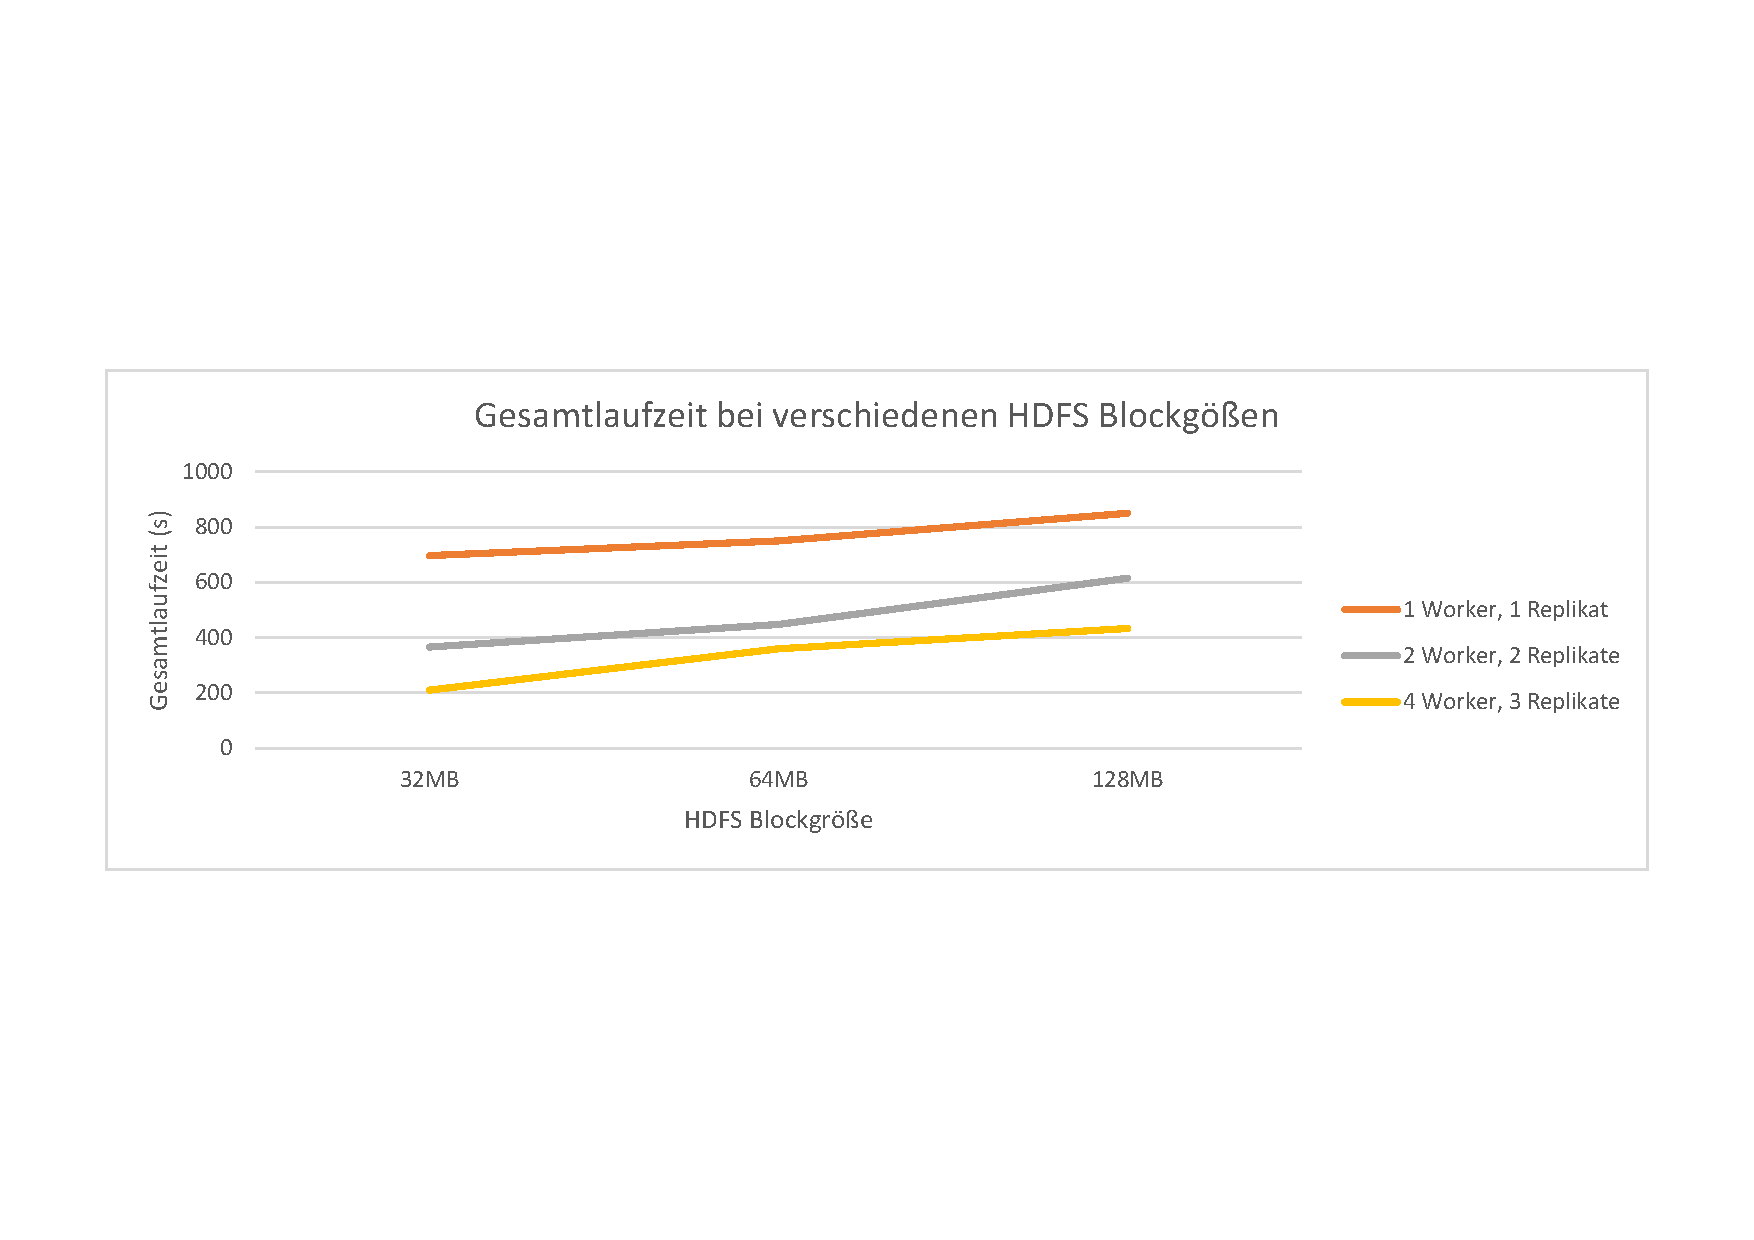
\includegraphics[width=\textwidth]{runtime_vs_blocksize.pdf}
	\caption{Laufzeit der Feature Extraction bei unterschiedlichen HDFS Blockgrößen}
	\label{figure:runtime_vs_blocksize}
\end{figure}

Ein Hinweis auf den Flaschenhals bei der Verarbeitung auf einem einzigen Knoten ist in Abbildung~\ref{figure:1W32B1R_net_cpu} zu erkennen. Die CPU steht unter Volllast, während die Leistung beim Lesen von der SD-Karte mit durchschnittlich 4,3 MB/s deutlich unter dem möglichen Durchsatz bleibt (siehe Tabelle~\ref{table:worker_harddrive}).\\
Netzwerkdurchsatz spielt hier - wie bei einem einzelnen Knoten zu erwarten - offenbar keine Rolle.

\begin{figure}[ht!]
	\centering
  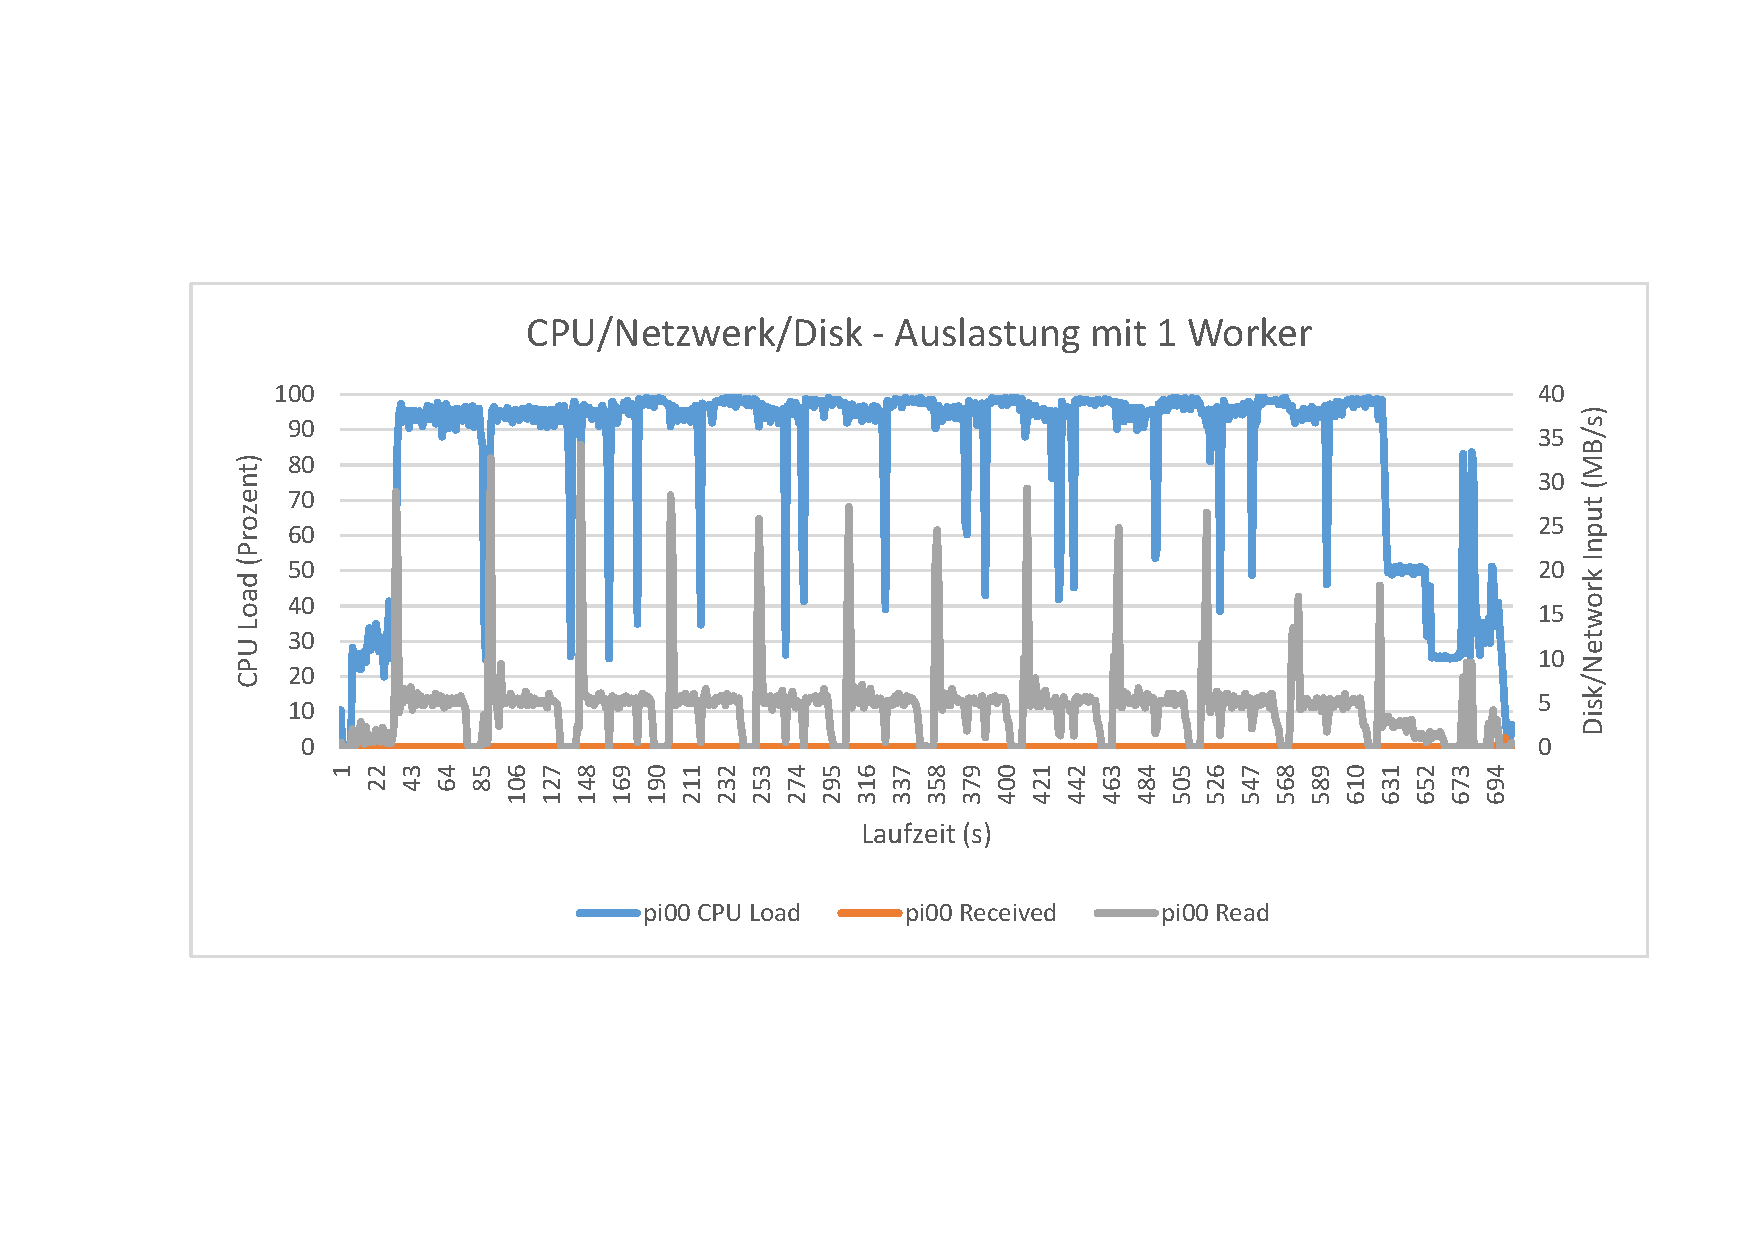
\includegraphics[width=\textwidth]{1W32B1R_net_cpu.pdf}
	\caption{Netzwerk-, SD-Karten und CPU-Auslastung während bei einem Worker und 32MB Blockgröße}
	\label{figure:1W32B1R_net_cpu}
\end{figure}

Betrachtet man die Summe der IO-Durchsätze über sämtliche Knoten lassen sich deutlich die verschiedenen Phasen der Feature-Extraction erkennen. Abbildung~\ref{figure:4W64B2R_io} zeigt das kommentierte Diagramm eines Testlaufs mit 4 Workern, 2 Replikaten und einer HDFS-Blockgröße von 64MB.

\begin{figure}[ht!]
	\centering
  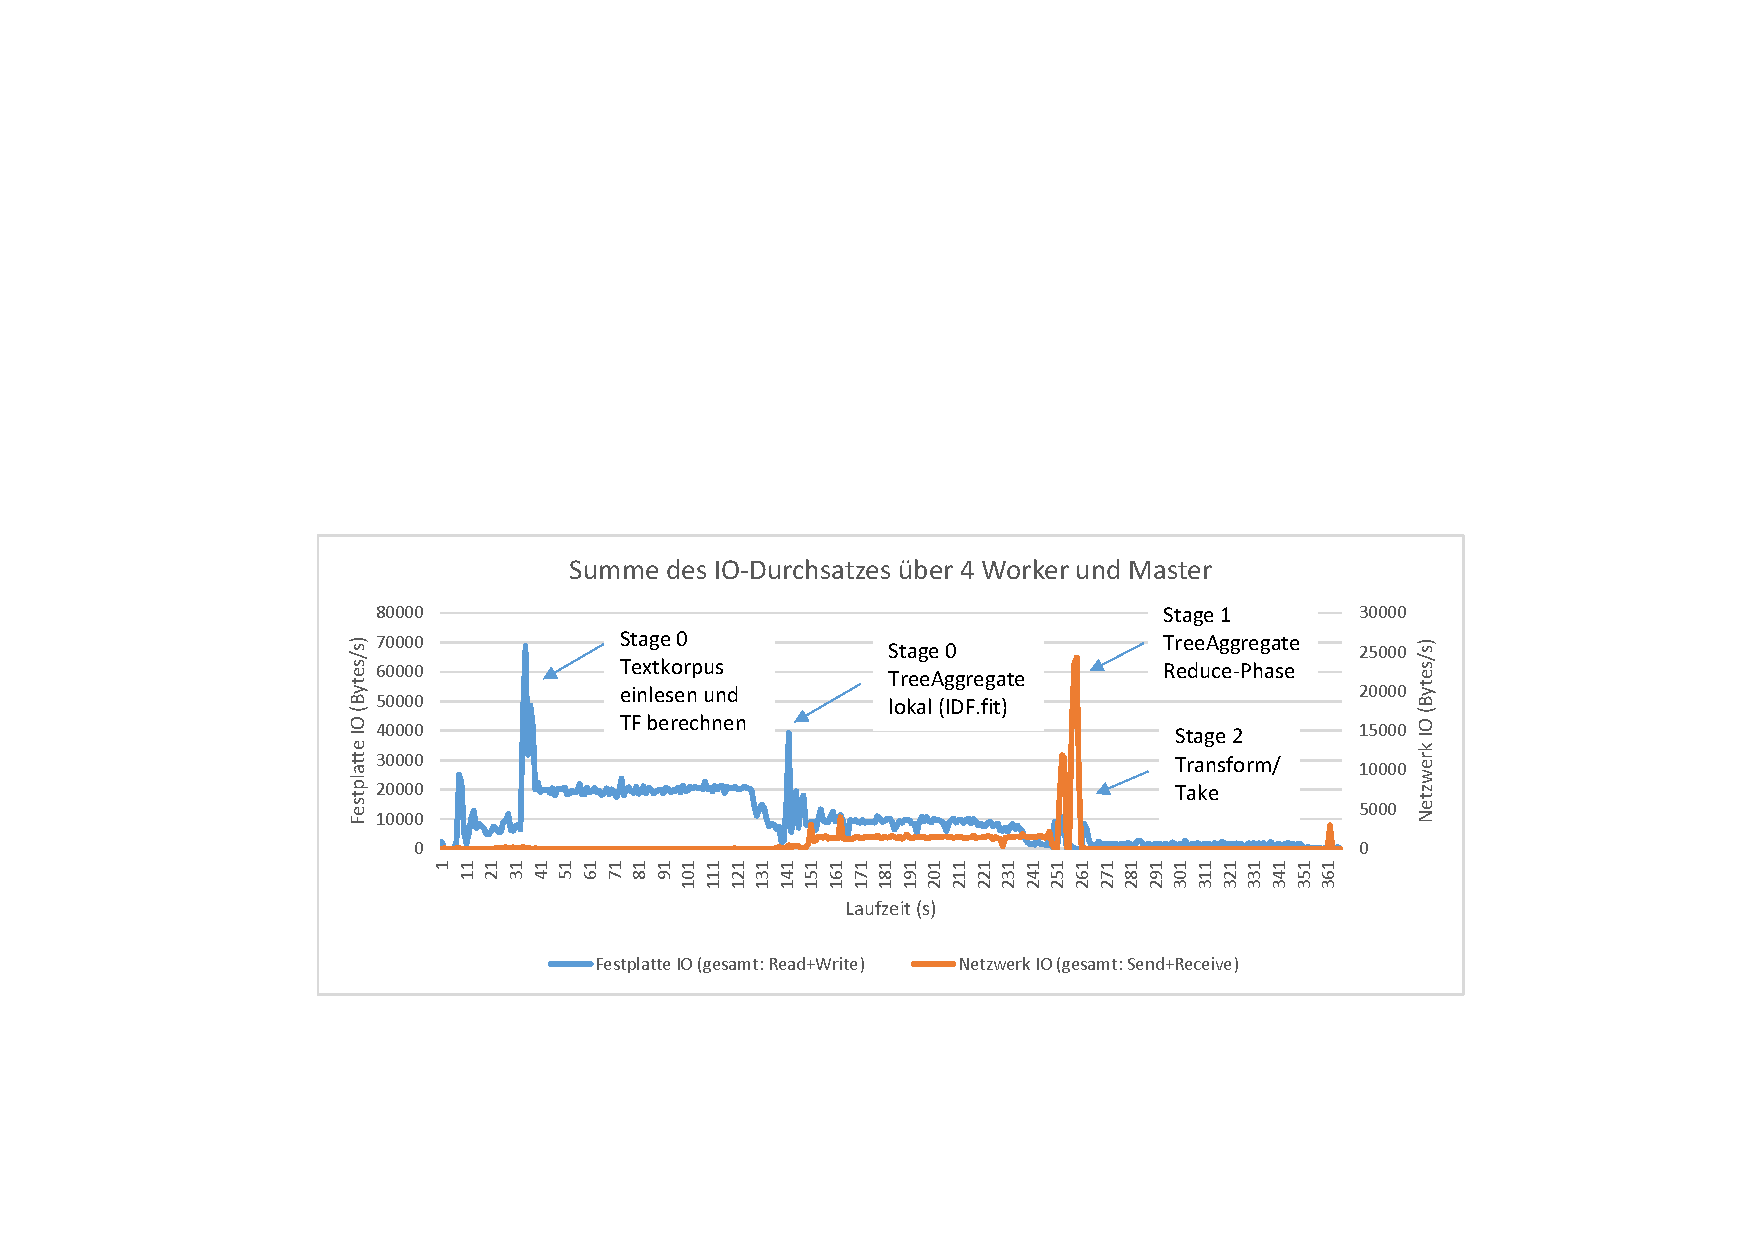
\includegraphics[width=\textwidth]{4W64B2R_io.pdf}
	\caption{Auslastungskurven bei einem Worker und 64MB Blockgröße}
	\label{figure:4W64B2R_io}
\end{figure}

\begin{labeling}{Anmerkung:~}
\item[Anmerkung:] Die Methode \lstinline|treeAggregate|\footnote{https://github.com/apache/spark/blob/branch-1.3/core/src/main/scala/org/apache/spark/rdd/RDD.scala\#L978} stellt einen Spezialfall unter den \gls{rdd}-
Transformationen dar. Sie besteht aus zwei Phasen, wobei in der ersten Phase lokal auf den Partitionen eine Aggregation von Datensätzen durchgeführt wird anschließend über \lstinline|reduce| die partitionsübergreifende Aggregation der bereits partiell aggregierten Datensätze durchgeführt wird.\\
Aus dieser Implementation ergibt sich die Netzwerk-Lastspitze innerhalb von Stage 1 (Abb.~\ref{figure:4W64B2R_io}).
\end{labeling}

\subsection{Echtzeitkomponente}

Einen ersten Blick auf den Zustand einer Spark-Anwendung ermöglicht die Weboberfläche des Treibers.\\

Jede Spark-Applikation startet gemäß der Standardeinstellungen auf dem Host des Treibers einen HTTP-Server, über den verschiedene Daten verfolgt werden können. In Abb.~\ref{figure:realtime_dashboard_stats}) sind die Statistiken einer laufenden Realtime-Komponente dargestellt.\\

In dem betrachteten Fall läuft die Realtime-Komponente mit einem einzelnen Worker, der den Empfänger für den Datenstrom von Twitter startet und das Scoring und Filtern der eingehenden Nachrichten ausführt. Um den Worker nicht für die Modellerzeugung der Batch-Komponente zu blockieren, wurde nur ein Executor mit 2 Cores gewährt.

\begin{figure}[ht!]
	\centering
	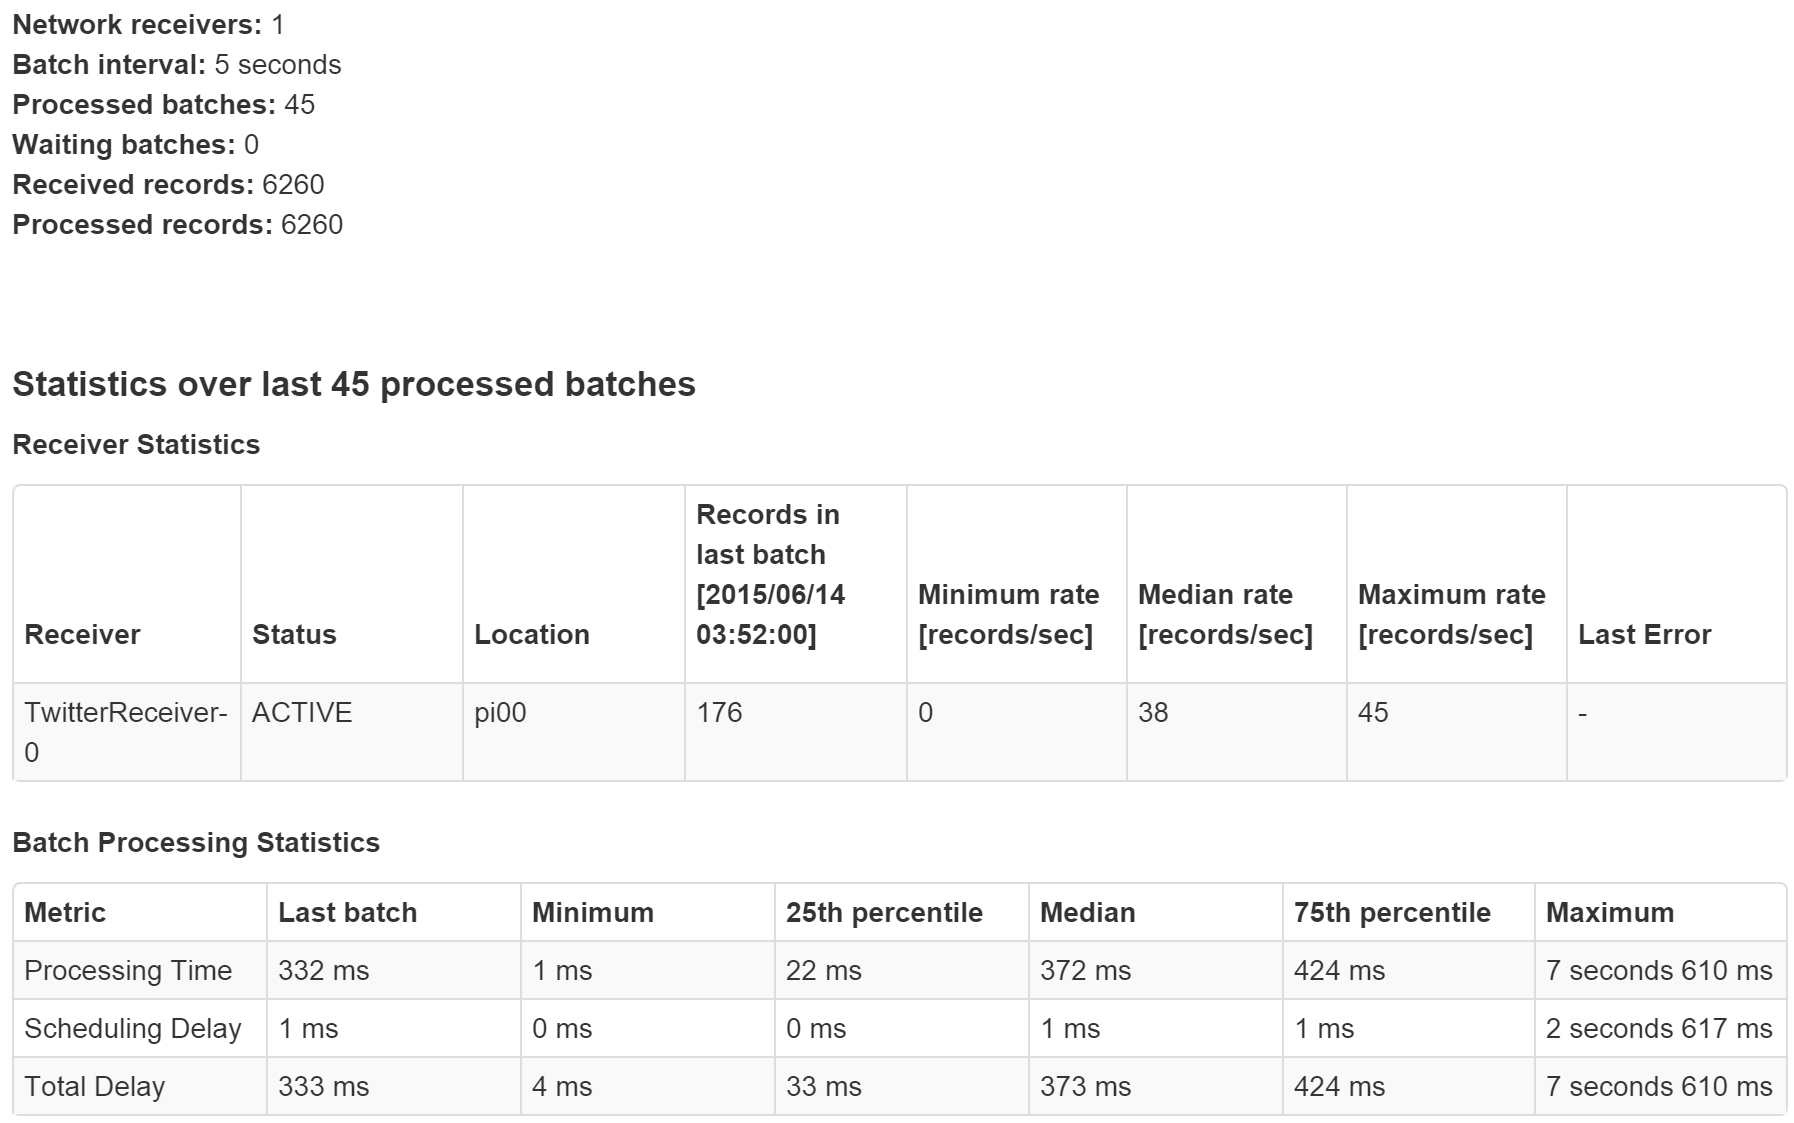
\includegraphics[width=\textwidth]{bilder/streaming_stats_dashboard.PNG}
	\caption{Spark-Dashboard des Realtime Analyzers - Statistics Tab}
	\label{figure:realtime_dashboard_stats}
\end{figure}

Zum Zeitpunkt des Schnappschusses wurden 6260 Tweets empfangen und verarbeitet. Der letzte Batch enthielt 178 Twitter-Nachrichten (im Durchschnitt sind es etwa 200) und der Median für die Verarbeitungszeit liegt bei 373 Millisekunden (\textit{Total Delay}.\\

Bei einem Zeitfenster von 5 Sekunden (\textit{Batch Interval}) pro Batch gibt es also keinen Hinweis auf Performanceprobleme bei der Verarbeitung.\\

Dieser Verdacht erhärtet sich bei einem Blick auf die CPU-Last des verarbeitenden Workers (Abb.~\ref{figure:str_1W_cpu}). Die durchschnittliche Last über den beobachteten Zeitraum liegt bei 22,5\%. Die Last des Master sogar nur bei 8,1\%.

\begin{figure}[ht!]
	\centering
	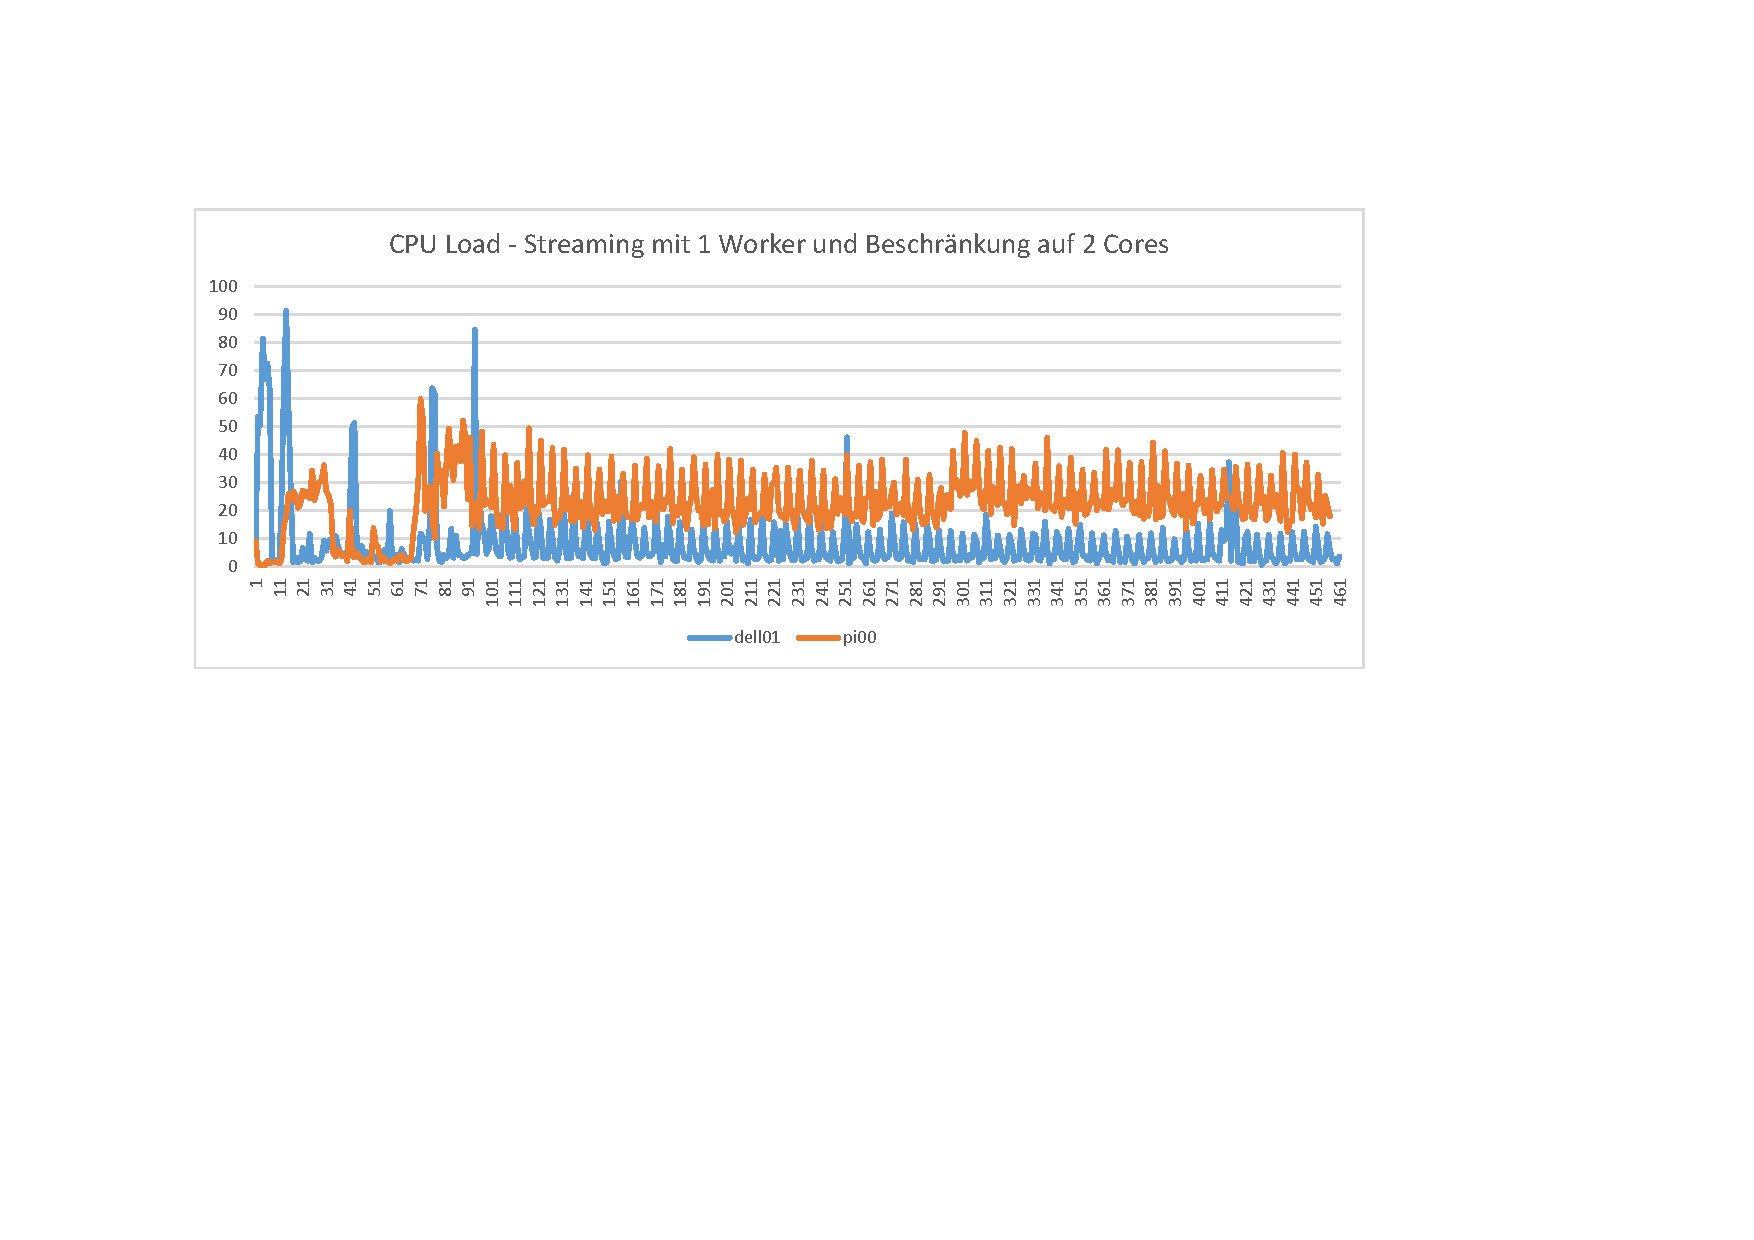
\includegraphics[width=\textwidth]{str_1W_cpu.pdf}
	\caption{CPU Last eines einzelnen Workers}
	\label{figure:str_1W_cpu}
\end{figure}

Auch die Netzwerklast ist minimal (Abb.~\ref{figure:str_1W_net}). Ab Sekunde 51 liegt die Last des Workers bei durchschnittlich 77 KByte/s. Über den beobachteten Zeitraum von knapp 7 Minuten wurden damit 31.4 Megabyte empfangen. Die Last des Masters liegt noch darunter.

\begin{figure}[ht!]
	\centering
	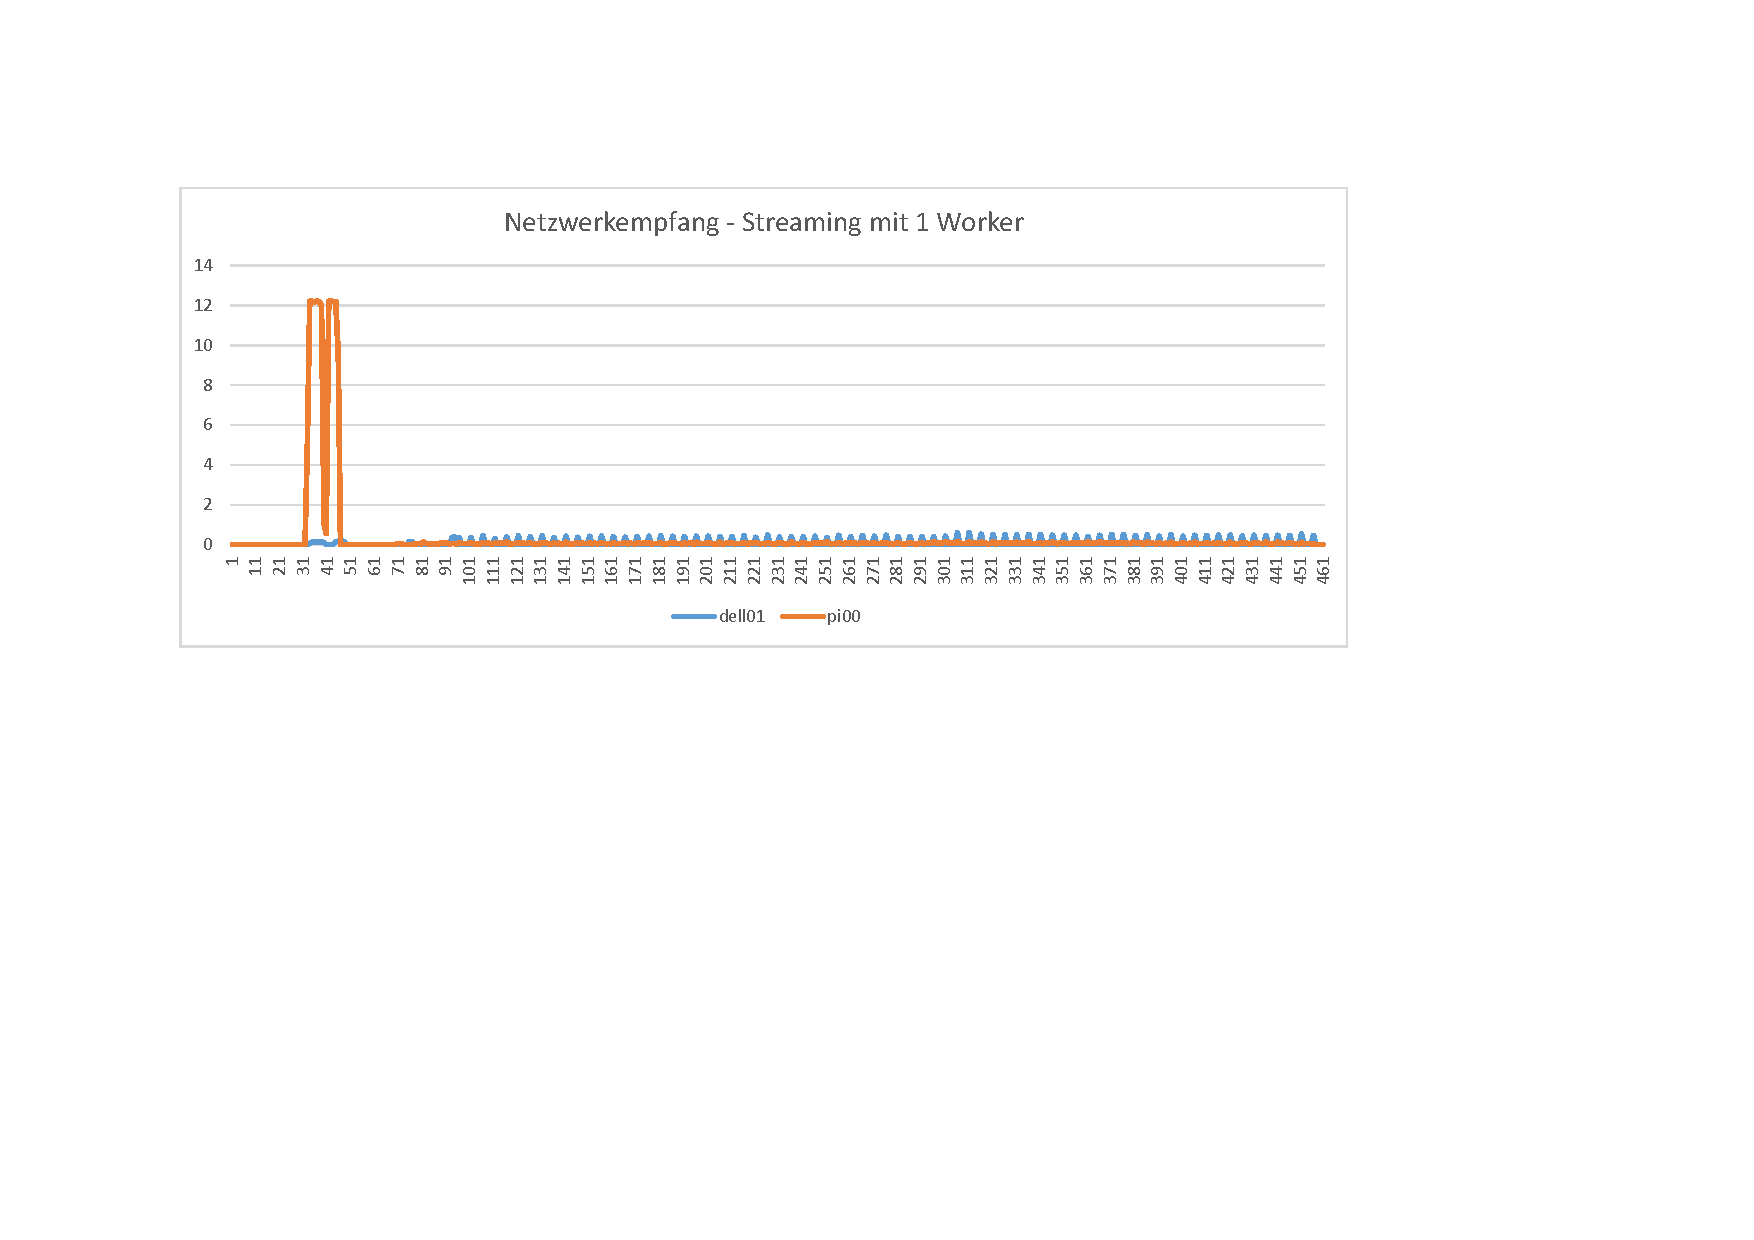
\includegraphics[width=\textwidth]{str_1W_net.pdf}
	\caption{CPU Last eines einzelnen Workers}
	\label{figure:str_1W_net}
\end{figure}

Betrachtet man den Speicherverbrauch (Abb.~\ref{figure:str_mit_mem_pi00}), sieht man, dass sich dieser nach wenigen Sekunden bei etwa 362MB stabilisiert.

\begin{figure}[ht!]
	\centering
	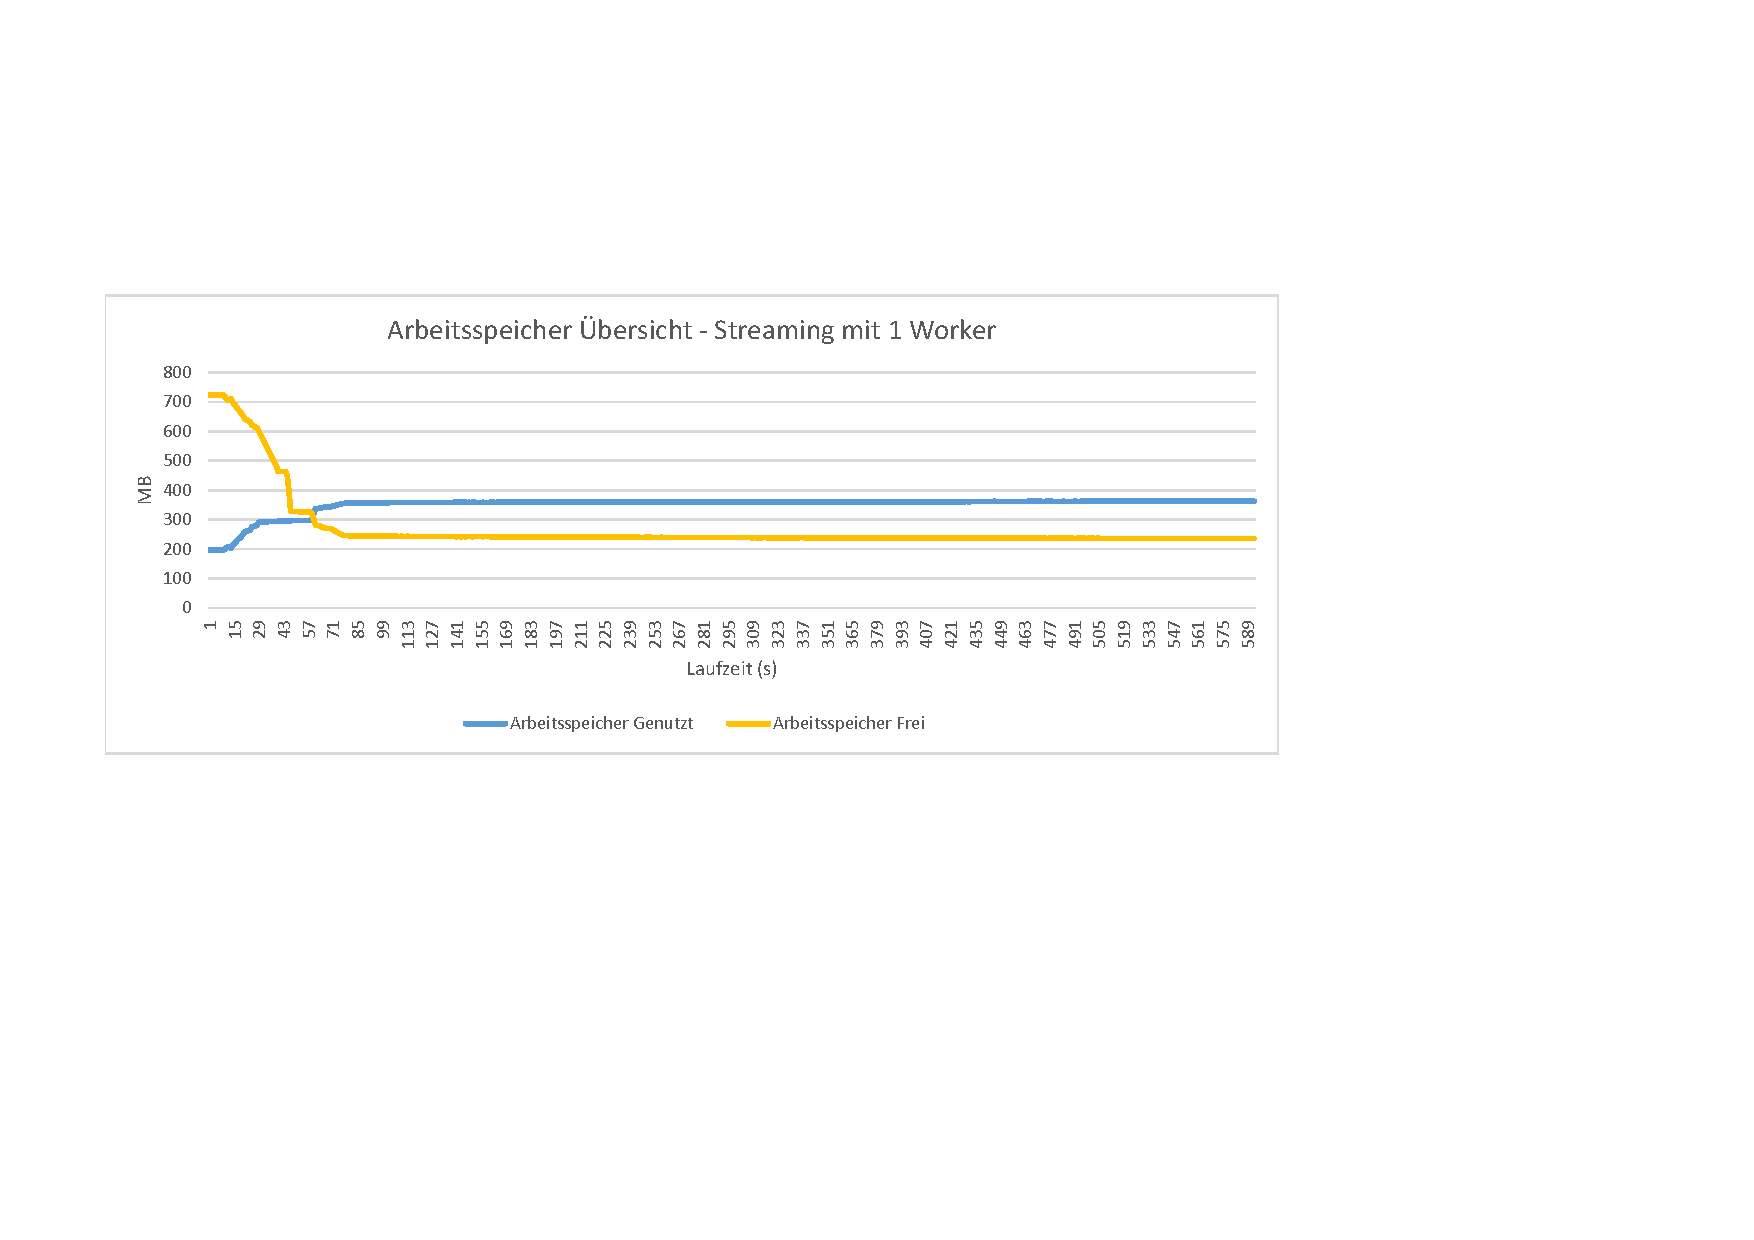
\includegraphics[width=\textwidth]{str_mit_mem_pi00.pdf}
	\caption{CPU Last eines einzelnen Workers}
	\label{figure:str_mit_mem_pi00}
\end{figure}

\subsection{Funktionale Qualität der Lösung}

\chapter{Schlussbetrachtung}
\section{Diskussion der Ergebnisse}
Es wurde ein umfassender Einblick in die Konzepte und Komponenten von Apache Spark gegeben. Für dieses System wurde daraufhin eine Anwendung entworfen und implementiert, die einen Echtzeitdatenstrom nach vorgegebenen Kriterien analysiert und dabei dynamisch auf geänderte Vorgaben reagieren kann.\\
Diese Anwendung wurde anschließend als Testfall für den Betrieb einer Apache Spark/Hadoop-Umgebung auf einem Low-End-Hardware-Cluster aus Raspberry Pis genutzt und das Laufzeitverhalten untersucht.\\

Dieses Experiment war erfolgreich. Es ist möglich einen Spark/Hadoop-Cluster auf der beschriebenen Hardware zu installieren und die genannte Anwendung stabil zu betreiben.\\

Dabei hat sich die Hardware sogar als leistungsfähiger als nötig erwiesen. Zwar profitiert insbesondere die Batch-Komponente deutlich von dem Hinzufügen weiterer Knoten, die Streaming-Komponente ist jedoch mit einem einzelnen Knoten bereits problemlos zu betreiben und erfährt durch verteilte Ausführung keine weitere Verbesserung der Performance.\\

Die geringe Last des kostenlosen Twitterdatenstroms verursacht für die weitere Bewertung der Ergebnisse zwei Probleme:
\begin{enumerate}
	\item Da selbst ein einzelner Knoten für die Analyse des Datenstroms mehr als ausreichend ist, lassen sich aus dem Experiment keine Aussagen über das Skalierungsverhalten der entsprechenden Komponente treffen.
	\item Bei der Exploration mehrerer zehntausend Tweets wurde kein einziger mit einem plausiblen Bezug zu den in der Spark-Mailingliste diskutierten Themen gefunden. Eine empirische Bewertung der funktionalen Qualitäten der Implementation ist damit nicht ohne Weiteres möglich.
\end{enumerate}

\section{Ausblick und offene Punkte}
Der Betrieb eines Spark/Hadoop-Clusters ist komplex. In dieser Arbeit wurde die Anwendungsentwicklung mit Spark und die Machbarkeit des Betriebs auf Low-End-Hardware behandelt. Für einen produktiven Betrieb der hier vorgestellten Architektur gibt es eine Reihe von Maßnahmen, die im Rahmen der betrachteten Fragestellungen ausgeblendet wurden:\\

\begin{enumerate}
	\item \textbf{Message Queues:} Für die robuste Verbindung zur asynchronen Kommunikation zwischen Batch- und Realtime-Komponente käme eine Erweiterung mt Messagequeues oder auch (NoSQL-)Datenbanken in Frage.
	\item \textbf{Umfangreichere Datenquellen:} Um die Skalierbarkeit der Streaming-Komponente unabhängig vom dem hier behandelten Anwendungsfall zu betrachten, könnte man einen eigenen speziellen Receiver implementieren und diesen mit einer kontrollierbaren Datenquelle verbinden. \textit{Kontrollierbar} heißt hier, dass die erzeugte Last flexibel erhöht werden kann, um die Kapazität des empfangenden Knotens zu übertreffen und eine verteilte Verarbeitung zu erzwingen.
	\item \textbf{Clustermanagement:} Die Konfiguration der Knoten und der verteilten Komponenten wurde für diesen Versuch überwiegend manuell durchgeführt. Um auch eine höhere Anzahl von Knoten verwalten zu können wären Werkzeuge zur Automatisierung von Konfiguration (z.B. Chef\footnote{https://www.chef.io/chef/}, Puppet\footnote{https://puppetlabs.com/}) oder Provisionierung (z.B. Docker\footnote{https://www.docker.com}, Rocket\footnote{https://github.com/coreos/rkt}, Kubernetes\footnote{http://kubernetes.io/}) notwendig.\\
	Für ein komfortables Monitoring könnte man den Cluster mit Tools zur dauerhaften Überwachung ausstatten (z.B. Nagios/Icinga\footnote{https://www.icinga.org/}, Ganglia\footnote{http://ganglia.sourceforge.net/}).
\end{enumerate}

Neben dem Betrieb der Anwendung, gibt es auch funktionale Aspekte die für eine produktive Anwendung erweitert werden könnten:

\begin{enumerate}
	\item \textbf{Textkorpus:} Als Textkorpus für das TF-IDF-Verfahren wurde für diesen \textit{Proof of Concept} der vervielfachte Inhalt von Nachrichten aus der Spark-User-Mailingliste verwendet (etwa 13000 Emails). Eine schärfere Abgrenzung relevanter Begriffe lässt sich wahrscheinlich durch einen unabhängigen Korpus erreichen (beispielsweise Wikipedia\footnote{http://www.wikipedia.org/} oder der klassische Reuters-Nachrichtenkorpus\footnote{https://kdd.ics.uci.edu/databases/reuters21578/reuters21578.html, abgerufen am 01.06.2015}).
	\item \textbf{Ähnlichkeitsmaß:} Das Scoring könnte darüber hinaus durch leistungsfähigere Verfahren verbessert werden - etwa durch Ähnlichkeitsmaße (\cite{Huang:2008}), die auch Synonyme erkennen.
	\item \textbf{Grafische Benutzeroberfläche:} Damit die gefilterten Nachrichten ihren Weg zum Benutzer finden, gibt es eine Vielzahl an Möglichkeiten. Naheliegend wäre ein Webinterface (z.B. über den MEAN-Stack\footnote{http://mean.io/#!/} oder das Play-Framework\footnote{https://www.playframework.com/} für Scala/Java).
\end{enumerate}
%\newglossaryentry{repl}{
name=Read Evaluate Print Loop,
description={Pattern zum Erzeugen einer Konsole, die in einer Endlosschleife Eingaben liest, die auswertet und das Ergebnis wieder ausgibt}
}

\newglossaryentry{sla}{
name=Service Level Agreement,
description={Übereinkunft zwischen dem Anbieter und dem Nutzer eines Dienstes über dessen Qualität (z.B. Antwortzeiten, Durchsatz, Verfügbarkeit, etc.)}
}

\newacronym{tst}{TST}{Test Test Test}


% bibliography and other stuff
\backmatter

\typeout{===== Section: literature}

%% Glossar
\newpage
\glstoctrue
\printglossary[title=Acronyme,toctitle=Acronyme,type=\acronymtype]
\printglossary[title=Glossar, toctitle=Glossar]

%% appendix
\typeout{===== File: appendices}
\newpage
\clearpage
\appendix
\begin{appendices}
\section{Installation der Plattform}
\section{Quellcode/Skripte (Auszüge)}
\subsection{Performance-Messungen}

\begin{lstlisting}[caption={Messung der Festplattenperformance - Beispiel: Schreiben einer 512MB Datei},label={lst:measure_harddrive}]
echo 3 > /proc/sys/vm/drop_caches
dd if=/dev/zero of=test512.out bs=512MB count=1
\end{lstlisting}

\begin{lstlisting}[caption={Messung der Netzwerkperformance},label={lst:measure_network}]
iperf -c <IP-Adresse des Peers> -r -P 4
\end{lstlisting}

\subsection{Monitoring}

\begin{lstlisting}[caption={Monitoring des Clusters (Betriebssystem), Beispiel ModelBuilder},label={lst:monitor_cluster}]
#/bin/bash

### ModelBuilder Wrapper Skript

TIME=`date +"%H-%M"`
WORKERS="pi00 pi01 pi02 pi03"

# Start Monitoring
	
for host in $WORKERS; do
  ssh $host "screen -d -m dstat -cdlsmn --output $1.log"
done
screen -d -m dstat -cdlsm --output $1.log

# Run App
/home/daniel/start_modelbuilder.sh $1-$TIME 2>&1 > \
  ~/metrics/$1_$TIME.log 

# Stop Monitoring
for host in $WORKERS; do
  ssh $host 'screen -X quit'
done
screen -X quit

# Collect results
for host in $WORKERS; do
  scp $host:/home/daniel/$1.log ~/metrics/dstat/$1_$host_$TIME.csv
done
cp ~/$1.log ~/metrics/dstat/$1_dell01_$TIME.csv

# Clean up
for host in $WORKERS; do
  ssh $host "rm /home/daniel/$1.log"
done
\end{lstlisting}

\subsection{Realisierung einer einfachen Continuous Deployment Pipeline}\label{subsec:pipeline}
\textit{post-receive}-Hook von dem Git-Repository\footnote{https://git-scm.com/, abgerufen am 06.06.2015} der ModelBuilder-Komponente
\begin{lstlisting}[caption={Einfache Continuous Deployment Pipeline. Beispiel: ModelBuilder},label={lst:cdp_modelbuilder}]
#/bin/bash

export SPARK_HOME=/opt/spark/

# clean up previous build
rm -rf ~/autobuilds/model_builder
cd ~/autobuilds
git clone ~/git/model_builder
cd model_builder

# run build
sbt package
if [ $? -ne "0" ]; then exit 1; fi

# run test suite
sbt test
if [ $? -ne "0" ]; then exit 1; fi

# deploy to cluster
/opt/spark/bin/spark-submit --class "de.haw.bachelorthesis.dkirchner\
.ModelBuilder" --master spark://192.168.206.131:7077 --driver-memory\
256m --executor-memory 384m \
~/autobuilds/model_builder/ [...] /model-builder_2.10-1.0.jar\
hdfs://192.168.206.131:54310/user/daniel/user_emails_corpus1.txt\
<emailaccount> <passwort>
\end{lstlisting}

\section{Konfigurationen}

\begin{lstlisting}[caption={hdfs-site.xml (Auszug): Beispiel mit Replikationsfaktor 1 und Blockgröße 32MB},label={lst:hdfs_config}]
<configuration>
  <property>
    <name>dfs.replication</name>
    <value>1</value>
  </property>
  <property>
    <name>dfs.block.size</name>
    <value>33554432</value>
  </property>
  <property>
    <name>dfs.permissions</name>
    <value>false</value>
  </property>
  <property>
    <name>dfs.datanode.drop.cache.behind.writes</name>
    <value>true</value>
  </property>
  <property>
    <name>dfs.namenode.datanode.registration.ip-hostname-check</name>
    <value>false</value>
  </property>
</configuration>
\end{lstlisting}

Eine vollständige Liste der HDFS-Optionen und -Standardeinstellungen kann unter [\footnote{https://hadoop.apache.org/docs/r2.7.0/hadoop-project-dist/hadoop-hdfs/hdfs-default.xml, abgerufen am 03.06.2015}] eingesehen werden.

\begin{lstlisting}[caption={spark-defaults.conf (Auszug)},label={lst:hdfs_config}]
spark.master                     spark://dell01:7077
spark.eventLog.enabled           true
spark.eventLog.dir               file:///home/spark/metrics/secondary
spark.shuffle.memoryFraction     0.3
\end{lstlisting}

\section{Sonstiges}
\subsection{Einschätzung des theoretischen Spitzendurchsatzes von Mittelklasse-Servern}
\label{subsec:commodity_servers}
Um zu einer groben Einschätzung des möglichen Datendurchsatzes verschiedener Schnittstellen bei "`Commodity Servern"' zu gelangen, wurden drei Systeme von großen Herstellern ausgewählt.\\
In der Grundkonfiguration kosten diese Systeme (zum Zeitpunkt dieser Arbeit) um die € 2000,- und lassen damit auf die Größenordnungen bei dem Datendurchsatz bestimmter Schnittstellen bei preisgünstigen Mehrzweck-Rechenknoten schließen.

\begin{table}[ht]
	\centering % used for centering table
	\begin{tabular}{c c c c} % centered columns (4 columns)
		\hline\hline %inserts double horizontal lines
		Modell & Netzwerkschnittstelle & Festspeicher & Arbeitsspeicher\\ [0.5ex] % inserts table
		%heading
		\hline % inserts single horizontal line
		Dell PowerEdge R530 & 1Gb/s Ethernet & PCIe 3.0 & DDR4\\ 
		HP Proliant DL160 Gen8 & 1Gb/s Ethernet & PCIe 3.0 & DDR3\\ 
		System x3650 M5 & 1Gb/s Ethernet & PCIe 3.0 & DDR4\\ % inserting body of the table
		\hline %inserts single line
	\end{tabular}
	\caption{Theoretische Spitzenleistungen bei Mehrzweck-Servern der 2000 Euro Klasse} % title of Table
	\label{table:vglinterfaces} % is used to refer this table in the text
\end{table}

Mit \cite{PCI14} und \cite{Fuj11} lassen sich grobe obere Abschätzungen errechnen, die in Tabelle~\ref{table:vgldurchsatz} angegeben sind.

\end{appendices}

%% read the documentation for customizing the style
%\bibliographystyle{dinat}
%\bibliography{sample}
\printbibliography

%\typeout{===== Section: nomenclature}
%% uncomment if a TOC entry is needed
%\addcontentsline{toc}{chapter}{Glossar}
%\renewcommand{\nomname}{Glossar}
%\clearpage
%\markboth{\nomname}{\nomname} %% see nomencl doc, page 9, section 4.1
%\printnomenclature

%% index
\newpage
\typeout{===== Section: index}
\printindex

%% Versicherung
\newpage
\HAWasurency

\end{document}
